%% Template para dissertacao/tese na classe UFBAthesis
%% versao 1.0
%% (c) 2005 Paulo G. S. Fonseca
%% (c) 2012 Antonio Terceiro
%% (c) 2014 Christina von Flach
%% www.dcc.ufba.br/~flach/ufbathesis

%% Carrega a classe ufbathesis
%% Opcoes: * Idiomas
%%           pt   - portugues (padrao)
%%           en   - ingles
%%         * Tipo do Texto
%%           bsc  - para monografias de graduacao
%%           msc  - para dissertacoes de mestrado (padrao)
%%           qual - exame de qualificacao de mestrado
%%           prop - exame de qualificacao de doutorado
%%           phd  - para teses de doutorado
%%         * Media
%%           scr  - para versao eletronica (PDF) / consulte o guia do usuario
%%         * Estilo
%%           classic - estilo original a la TAOCP (deprecated) - apesar de deprecated, manter esse.
%%           std     - novo estilo a la CUP (padrao)
%%         * Paginacao
%%           oneside - para impressao em face unica
%%           twoside - para impressao em frente e verso (padrao)

% Atenção: Manter 'classic' na declaracao abaixo:
\documentclass[qual, classic, a4paper]{ufbathesis}

%% Preambulo:
\usepackage[utf8]{inputenc}

%\usepackage[authoryear]{natbib}
\usepackage{graphicx}
\usepackage{lipsum}
\usepackage{hyphenat}
\usepackage[usenames, dvipsnames, table]{xcolor}
\usepackage{booktabs}
\usepackage{pifont}
\usepackage{multirow}
\usepackage{listings} 
\usepackage{colortbl}
\usepackage{xfrac}
\usepackage[FIGTOPCAP]{subfigure}
\usepackage{tabularx}
\usepackage{ragged2e}
\usepackage{acronym}
\usepackage{float}
\usepackage{todonotes}
\presetkeys%
    {todonotes}%
    {inline,backgroundcolor=yellow}{}
    
\usepackage{blindtext}


% Siglas
\acrodef{AM}[AM]{{Aprendizado de Máquina}}
\acrodef{EMD}[EMD]{{Decomposição de Modo Empírico}}
\acrodef{RQA}[RQA]{{\textit{Recurrence Quantification Analysis}}}
\acrodef{FAPAR}[FAPAR] {{\textit{Fraction of Absorbed Photosynthesis Active Radiation}}}
\acrodef{DTW}[DTW] {{\textit {Dynamic  Time  Warping}}}
\acrodef{DE}[DE] {{Distância Euclidiana}}
\acrodef{EDR}[EDR]{{ \textit{ Edite  Distance  Real}}}
\acrodef{FCD}[FCD] {{\textit {Fluxo de Dados Contínuos}}}
\acrodef{DN}[DN] {{\textit {Detecção de Novidade}}}
\acrodef{CID}[CID]{{\textit{Complexity-Invariant Distance}}}
\acrodef{SLR}[SLR]{{\textit{Systematic  Literature  Review}}}
\acrodef{SANTS}[SANTS]{{\textit{Similarity Analysis on Nonstationary Time Series}}} 
\acrodef{MDDL}[MDDL]{{\textit{Mean Distance from the Diagonal Line}}}


% Universidade
\university{Universidade Federal da Bahia}

% Endereco (cidade)
\address{Salvador}

% Instituto ou Centro Academico
\institute{Instituto de Matem\'{a}tica}

% Nome da biblioteca - usado na ficha catalografica
\library{Biblioteca Reitor Mac\^{e}do Costa}

% Programa de pos-graduacao
\program{Programa de P\'{o}s-Gradua\c{c}\~{a}o em Ci\^{e}ncia da Computa\c{c}\~{a}o}

% Area de titulacao
\majorfield{Ci\^{e}ncia da Computa\c{c}\~{a}o}

% Titulo da dissertacao
\title{Aplicando redes de função de base radial para detecção de novidades em fluxos contínuos de dados}

% Data da defesa
% e.g. \date{19 de fevereiro de 2013}
\date{03 de Abril de 2019}
% e.g. \defenseyear{2013}
\defenseyear{2019}

% Autor
% e.g. \author{Jose da Silva}
\author{Ruivaldo Azevedo Lobão Neto}

% Orientador(a)
% Opcao: [f] - para orientador do sexo feminino
% e.g. \adviser[f]{Profa. Dra. Maria Santos}
\adviser{Ricardo Ara\'{u}jo Rios}

% Orientador(a)
% Opcao: [f] - para orientador do sexo feminino
% e.g. \coadviser{Prof. Dr. Pedro Pedreira}
% Comente se nao ha co-orientador
%\coadviser{Nome Completo do CO-ORIENTADOR}

%% Inicio do documento
\begin{document}

\pgcompfrontpage

%% Parte pre-textual
\frontmatter

\pgcomppresentationpage

%%%%%%%%%%%%%%%%%%%%%%%%%
% Ficha catalografica
%%%%%%%%%%%%%%%%%%%%%%%%%

%\authorcitationname{Silva, Mirlei Moura da } % e.g. Terceiro, Antonio Soares de Azevedo
%\advisercitationname{Sobrenome, Nome do ORIENTADOR} % e.g. Chavez, Christina von Flach Garcia
%\coadvisercitationname{Sobrenome, Nome do CO-ORIENTADOR} % e.g. Mendonca, Manoel Gomes de
%\catalogtype{Disserta\c{c}\~{a}o (Mestrado)} % e.g. ou ``Tese (Doutorado)''

%\catalogtopics{1. Primeira palavra-chave. 2. Segunda palavra-chave. 3. Terceira palavra-chave} % Listar palavras-chave do trabalho para a FICHA CATALOGRAFICA}, por exemplo, ``1. Complexidade Estrutural. 2. Qualidade de Software 3. Engenharia de Software''
%\catalogcdd{XXX.XX} % e.g.  XXX.XX (número nesse formato serah dado pela biblioteca)
%\catalogcdu{XXX.XX.XXX} % e.g.  XXX.XX.XXX (idem) 
%\catalogingsheet

%%%%%%%%%%%%%%%%%%%%%
% Termo de aprovacaoo
%%%%%%%%%%%%%%%%%%%%%

\approvalsheet{Salvador, 03 de Abril de 2019}{
   \comittemember{Prof. Dr. Ricardo Araújo Rios}{UFBA}  
   %\comittemember{Profa. Dr...}{UFBA}
   %\comittemember{Prof. Dr...}{USP} 
}
   % Para mestrado, apenas 3.
   % \comittemember{Prof. Dr. Professor 4}{Universidade HJKL}
   % \comittemember{Profa. Dra. Professora 5}{Universidade QWERTY}

%%%%%%%%%%%%%%%%%%%%%%%%%%%%%%%%%%%%%%%% 
% Dedicatoria, Agradecimentos, Epigrafe
%%%%%%%%%%%%%%%%%%%%%%%%%%%%%%%%%%%%%%%%

% Comente para ocultar
%\begin{dedicatory}
%DIGITE A DEDICATORIA AQUI
%\end{dedicatory}

% Agradecimentos
% Se preferir, crie um arquivo `a parte e o inclua via \include{}
%\acknowledgements
%DIGITE OS AGRADECIMENTOS AQUI

% Epigrafe
%\begin{epigraph}[NOTA]{AUTOR}
%DIGITE AQUI A CITACAO
%\end{epigraph}

%%%%%%%%%%%%%%%%%%%%%
% Resumo 
%%%%%%%%%%%%%%%%%%%%%
\resumo

\blindtext

% Palavras-chave do resumo em Portugues
\begin{keywords}
    Aprendizado de Máquina, fluxos contínuos de dados, Mudanças de Conceito, Redes de Função de Base Radial, Não supervisionado
\end{keywords}

\abstract

\blindtext

% Palavras-chave do resumo em Ingles
\begin{keywords}
    Machine Learning, Data Streams, Concept Drift, Radial Basis Function Networks, Unlabeled
\end{keywords}

%%%%%%%%%%%%%%%%%%%
% Sumario / Indice
%%%%%%%%%%%%%%%%%%%

% Comente para ocultar
\tableofcontents

% Lista de figuras
% Comente para ocultar
\listoffigures

% Lista de tabelas
% Comente para ocultar
\listoftables

%% Parte textual
\mainmatter

% Eh aconselhavel criar cada capitulo em um arquivo separado, digamos
% "capitulo1.tex", "capitulo2.tex", ... "capituloN.tex" e depois
% inclui-los com:
% \include{capitulo1}
% \include{capitulo2}
% ...
% \include{capituloN}
%
% Importante: 
% Use \xchapter{}{} ao inves de \chapter{}; se não quiser colocar texto antes do inicio do capitulo, use \xchapter{texto}{}.

%%%
\xchapter{Introdução}{} \label{introducao}

\section{Contexto e Motivação}
 
Vivemos em uma era cuja a velocidade e a quantidade de dados produzidos são enormes.
De acordo com relatório da IDC \cite{idc_report}, 
os dados gerados em 2014 eram estimados em 4,4 zettabytes (trilhões de gigabytes) e este número tendia a um crescimento exponencial. 
O mesmo relatório prevê que em 2020 este número será de 44 zettabytes.

Em muitos contextos, os dados são produzidos em sequências de registros, denominados \textbf{eventos}, 
disponíveis ao longo do tempo, em uma determinada ordem \cite{Feigenbaum:2003:ALD:589343.592594}. 
Essas séries de dados são normalmente de alta frequência e potencialmente infinitas.
Sendo denominadas como Fluxos Contínuos de Dados (FCDs).

Exemplos de aplicações que produzem FCDs incluem: transações enviadas por processadores de cartões de crédito, 
detecção de temperatura por centros de monitoramento climático, operações no mercado de ações, monitoramento do coração, 
etc \cite{Aggarwal:2003:FCE:1315451.1315460}.

Nos últimos anos, técnicas de aprendizado de máquina aplicadas a fluxos contínuos de dados têm se tornado um tema de interesse entre diversos pesquisadores.
A principal característica nestes cenários é a necessidade de respostas que atendam a severas restrições de tempo \cite{Gama:2010:KDD:1855075}. 
Por exemplo, um classificador deve fornecer um resultado para um determinado evento antes que o próximo ocorra. 
Caso isso não aconteça, alguns eventos podem ficar sem classificação.

Outra dificuldade encontrada nesses ambientes é a mudança na distribuição dos dados. 
Este problema é conhecido como mudança de conceito (\textit{concept drift}) \cite{Gama:2010:KDD:1855075}.
Estas mudanças são classificadas conforme a velocidade com que ocorrem.
Mudanças de conceito \textbf{abruptas} identificam transições rápidas entre conceitos. 
Transições mais lentas, são ditas \textbf{graduais}.

Para fins de exemplificação, suponhamos que o histórico de transações via cartão de crédito de determinado cliente seja armazenado.
Este cliente, ao longo de vários anos, utiliza o cartão apenas para comprar alimentos, sempre em uma mesma região da cidade.
A partir dessas informações, um modelo é construído.
Contudo, não é coerente considerar que esse perfil jamais será modificado. 

Diante deste contexto, devemos considerar as seguintes situações:
1) Abruptamente, esse cliente compra vários eletrônicos em outro país.
Neste caso, compete aos métodos de detecção identificar se houve uma fraude ou se o cliente está apenas viajando e aproveitando ofertas.
2) Gradualmente, o mesmo cliente passa a utilizar o cartão para compras de passagens aéreas e diminui paulatinamente a utilização para compra de alimentos.
Após certo período, o perfil de compra estará completamente renovado.
Assim, cabe novamente aos métodos de detecção identificar a mudança de comportamento e emitir um alerta, 
para que o modelo construído seja atualizado.

Diversas abordagens e algoritmos para detecção de mudanças de conceito foram propostos na literatura.
Cada uma dessas técnicas possui características e parâmetros diferentes que visam aumentar sua eficiência, 
conforme a natureza dos dados e do tipo de mudança que se deseja otimizar.
Essas técnicas geralmente utilizam os resultados de um ou mais classificadores para identificar a mudança de conceito.
A mudança é indicada quando a quantidade de erros de classificação supera os acertos a partir de uma determinada métrica.

Algoritmos que adotam esta abordagem incluem: 
DDM (GAMA et al., 2004), EDDM (BAENA-GARCíA et al., 2006), 
ADWIN (BIFET; GAVALDA, 2007), ECDD (ROSS et al., 2012), 
PL (BACH; MALOOF, 2008), FCWM (SEBASTIAO et al., 2010),
PHT (PAGE, 1954), STEPD (NISHIDA; YAMAUCHI, 2007) e DOF (SOBHANI; BEIGY,2011). 
Adicionalmente, (SEBASTIAO; GAMA, 2009) fazem um estudo comparativo entre alguns desses métodos e destacam vantagens e desvantagens em diferentes situações.

\section{Hipótese e Objetivo}

Considerando as observações da seção anterior, a seguinte hipótese foi elaborada:

\begin{center}
\textit{``A aplicação de redes de função de base radial sobre fluxos contínuos de dados, permite a detecção de mudanças de conceito, sem requerer manutenção de estados prévios, de forma ágil e com baixos requisitos de processamento.''}
\end{center}

O objetivo deste trabalho será o desenvolvimento e validação da hipótese.
Para tanto, será desenvolvido um algoritmo para detecção de mudanças de conceito baseado em redes de função de base radial. Este algoritmo diferencia-se por realizar a escolha do centros de forma \textit{online}, conforme novas entradas são recepcionadas e por apresentar um raio dinâmico. 
A ativação de novos centros é usado como indicador para possíveis mudanças de conceito.

O algoritmo implementado será comparado com o estado da arte. Os fluxos contínuos de dados utilizados nos experimento, serão divididas em dois conjuntos. Um conjunto formado por séries sintéticas, para análise das características métricas da técnica proposta. E outro conjunto, formado por datasets oriundos de aplicações de aprendizagem de máquina do mundo real que apresentam mudanças de conceito.

Este trabalho está organizado conforme a seguinte estrutura: O \textbf{Capítulo \ref{revisao_bibliografica}} possui uma revisão bibliográfica dos principais conceitos utilizados neste trabalho como, por exemplo, fluxos contínuos de dados, mudança de conceito e principais algoritmos; No \textbf{Capítulo \ref{plano_pesquisa}} o plano de pesquisa definido é detalhado, identificando a metodologia que será aplicada e o cronograma de atividades. Por fim, o \textbf{Capítulo \ref{experimentos_iniciais}}, apresenta um conjunto de experimentos preliminares e a análise dos resultados obtidos em relação ao estado da arte.

\xchapter{Revisão Bibliográfica}{} \label{revisao_bibliografica}
\section{Considerações Iniciais}

Nas próximas seção, introduziremos os campos de fluxos contínuos de dados e detecção de mudança de conceito, tópicos importante no escopo deste trabalho. Por fim, apresentamos trabalhos relacionados encontrados na literatura.

\section{fluxos contínuos de dados}

fluxos contínuos de dados podem ser definidos como sequências abertas de dados produzidos continuamente \cite{Pavlidis:2011:9AC:1860144.1860487}.
Normalmente, supõe-se que eles são produzidos em grandes volumes e em altas freqüências. Alguns sistemas do mundo real produzem fluxos contínuos de dados, como os associados à telecomunicação empresas, sistemas bancários, mercado de ações, redes de sensores, satélites meteorológicos, Grande Colisor de Hádrons, etc \cite{Guha:2003:CDS:776752.776777}.
Tais fluxos podem ser estudados e analisados continuamente, a fim de obter informações dos fenômenos responsáveis para gerá-los e, portanto, modelar e prever seu comportamento. No contexto desta tese, os fluxos contínuos de dados são representados como sequências de observações x1,. . . , XI , . . . , xn, em que cada a observação é um vetor de d atributos reais, isto é, xi E Rd.

Dada a alta frequência possível que os dados são produzidos, os algoritmos para processar streams sofrem restrições em sua complexidade de tempo, uma vez que o algoritmo não pode executar operações exigentes durante o processamento de cada observação de dados, caso contrário a análise do fluxo seria afetada \cite{EDDM}.

Outra restrição está associada à natureza infinita dos fluxos - uma vez que a memória do computador é limitada, apenas as informações de dados ou mais importantes devem ser armazenadas. Devido a essas duas restrições, os algoritmos do fluxo de dados devem analisar os dados coletados, armazenar suas características ou informações relevantes e descartá-los a seguir. Portanto, as observações de dados devem ser processadas em uma única passagem, ou seja, de uma maneira inteiramente diferente dos conjuntos de dados tradicionais, cujas observações são completamente armazenadas na memória e processadas várias vezes, como um lote.

\section{Mudança de Conceito}
\blindtext

\subsection{Algoritmos para Detecção de Mudança de Conceito}
\blindtext

\subsection{Ferramentas}
\blindtext

\section{Redes de Função de Base Radial}
\blindtext
  
\section{Trabalhos Relacionados}
\blindtext

\section{Considerações Finais}
\blindtext

\xchapter{Plano de Pesquisa}{} \label{plano_pesquisa}
\section{Considerações Iniciais}
\blindtext

\section{Descrição do Problema}
\blindtext

\subsection{Atividades de Pesquisa}
\blindtext

\section{Considerações Finais}
\blindtext

\xchapter{Experimentos Iniciais}{} \label{experimentos_iniciais}
\section{Considerações Iniciais}
\blindtext

\section{Configuração dos Experimentos}
\blindtext

\section{Método de Pettitt}
\blindtext

\section{Redes de Função de Base Radial}
\blindtext

\section{Considerações Finais}
\blindtext


%% Parte pos-textual
\backmatter

% Bibliografia
% É aconselhável utilizar o BibTeX a partir de um arquivo, digamos "biblio.bib".
% Para ajuda na criação do arquivo .bib e utilização do BibTeX, recorra ao
% BibTeXpress em www.cin.ufpe.br/~paguso/bibtexpress
\bibliographystyle{abntex2-alf}
\bibliography{biblio}

% Apendices
% Comente se naoo houver apendices
%\appendix

%\xchapter{Exemplo de Ap\^endice}{} %sem preambulo
%\lipsum
% Eh aconselhavel criar cada apendice em um arquivo separado, digamos
% "apendice1.tex", "apendice.tex", ... "apendiceM.tex" e depois
% inclui--los com:
%\xchapter{Decomposição das séries temporais}{} %sem preambulo
\label{apendice1}
\section{Considerações Iniciais}
Neste apêndice consta as 40 séries temporais utilizadas nos experimentos mostrados no Capitulo \ref{experimentos}. As séries foram divididas em 4 tipos conforme a Tabela \ref{series}, onde o tipo representa um conjunto de 10 séries senoide ou cossenoide, sendo acrescida de ruído ou acrescida de ruído e tendência.
Nas imagens são representadas, a séries original,   seu componente determinístico e seu componente estocástico, os quais foram extraídos após a decomposição.
\section{Séries TIPO 1}
10 séries cossenoide com ruído ao longo da série.
\graphicspath{{imagens/}}
\begin{figure}[H]
\begin{center}
  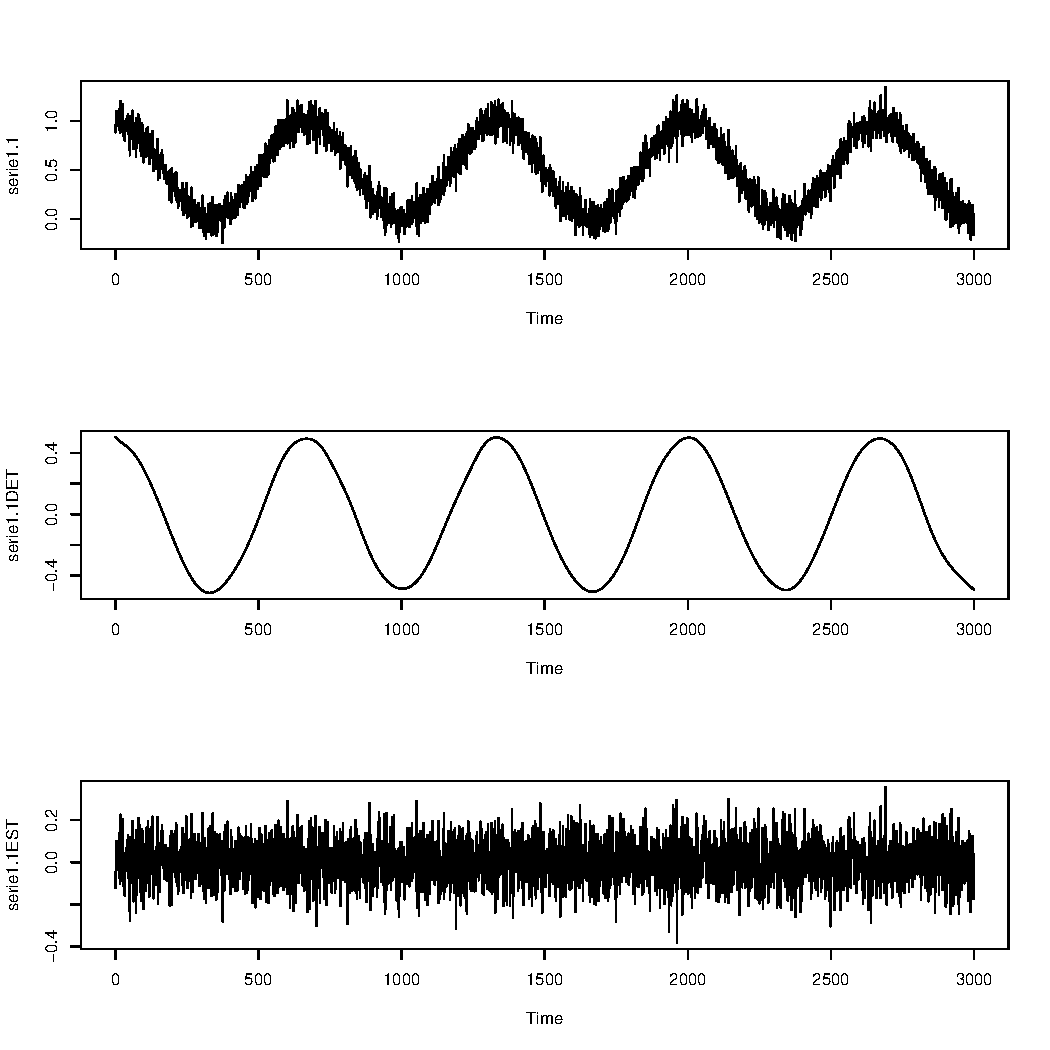
\includegraphics[scale=0.43]{serie1_1.pdf} \quad
  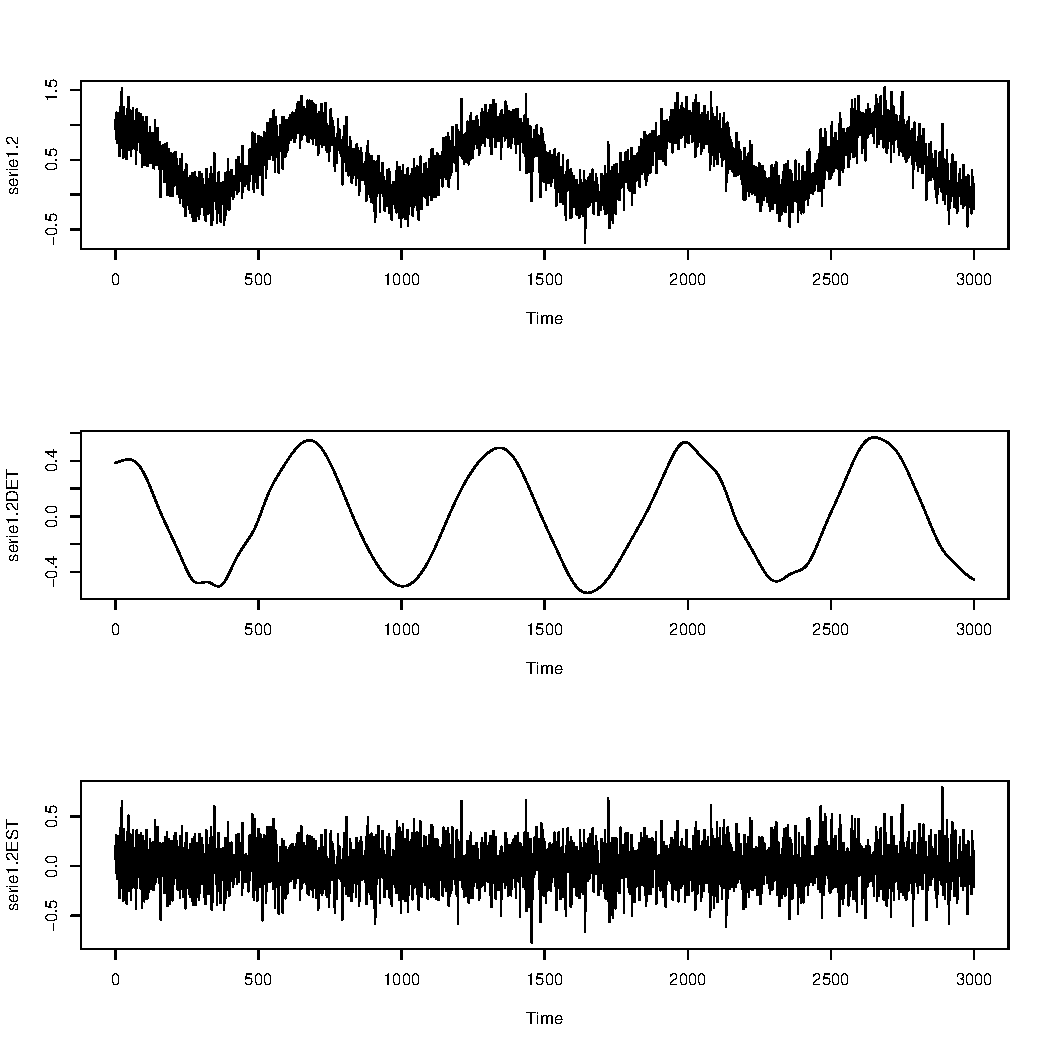
\includegraphics[scale=0.43]{serie1_2.pdf}
  \caption{Série 1.1 e Série 1.2}

\end{center}
\end{figure}

\graphicspath{{imagens/}}
\begin{figure}[H]
\begin{center}
  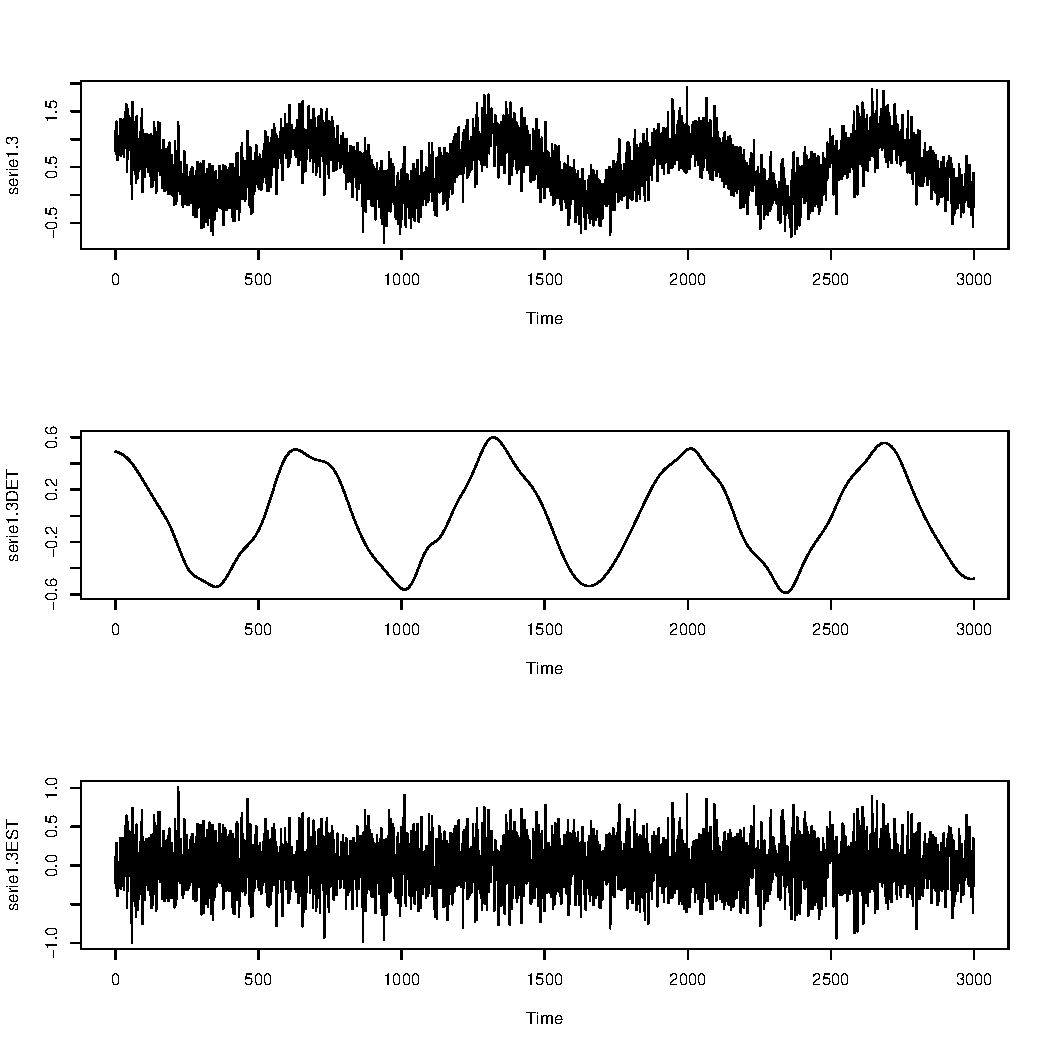
\includegraphics[scale=0.43]{serie1_3.pdf} \quad
  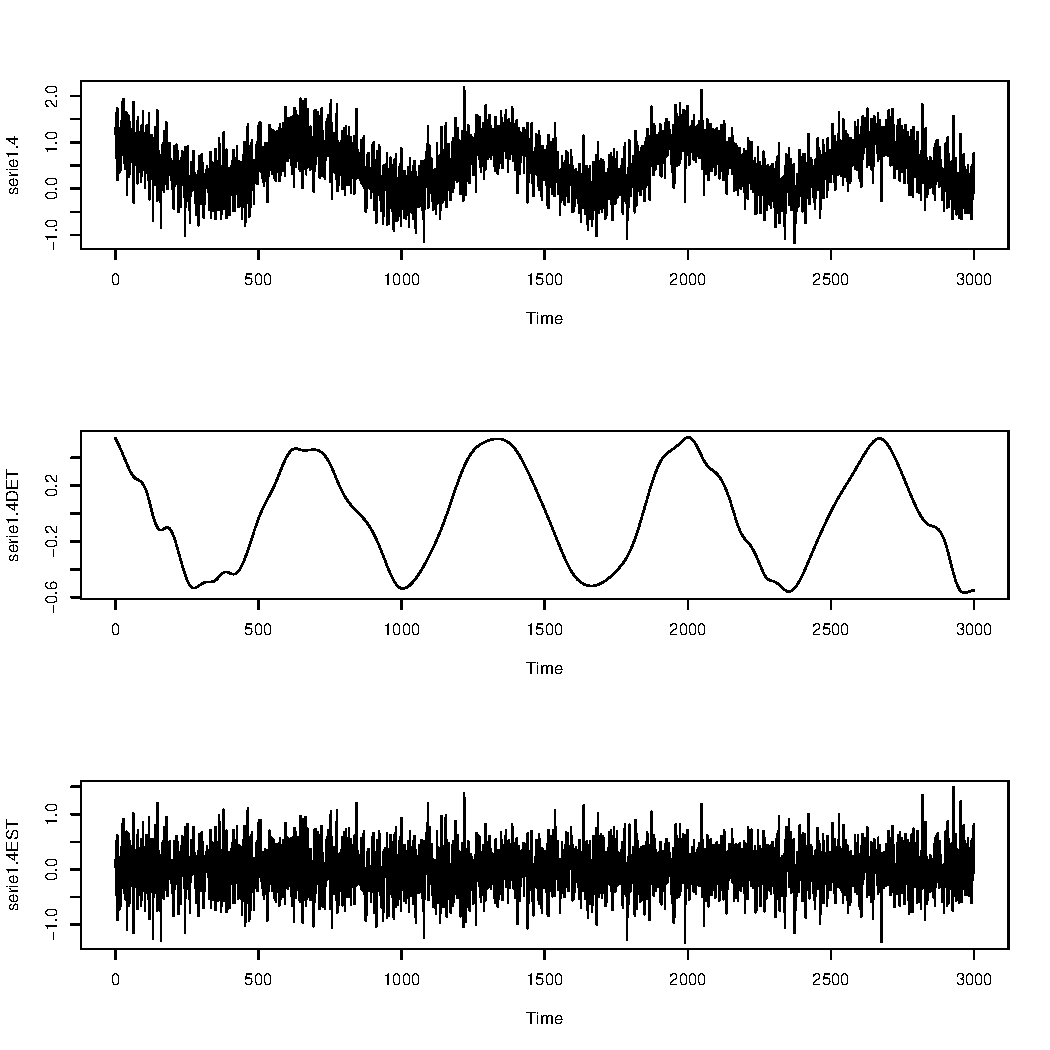
\includegraphics[scale=0.43]{serie1_4.pdf}
  \caption{Série 1.3 e Série 1.4}

\end{center}
\end{figure}

\graphicspath{{imagens/}}
\begin{figure}[H]
\begin{center}
  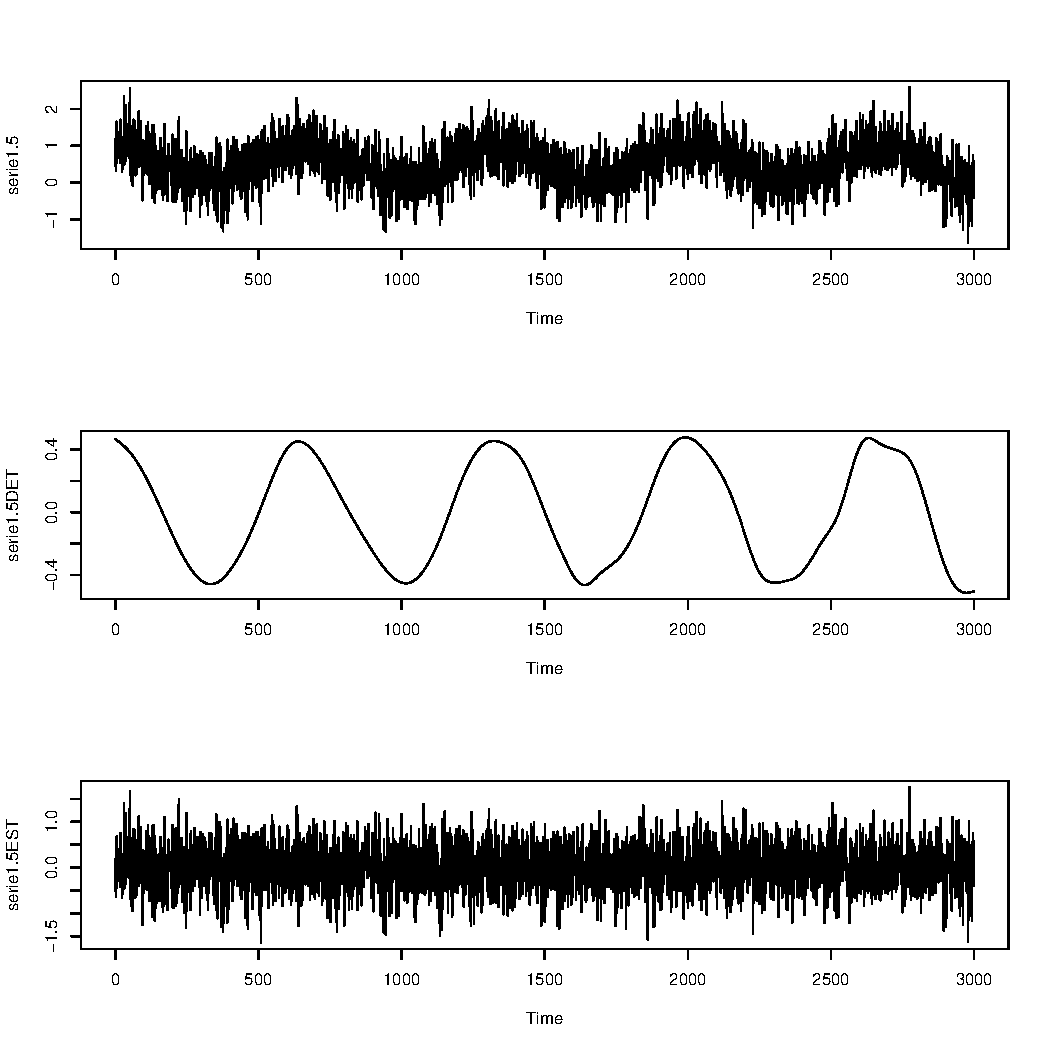
\includegraphics[scale=0.43]{serie1_5.pdf} \quad
  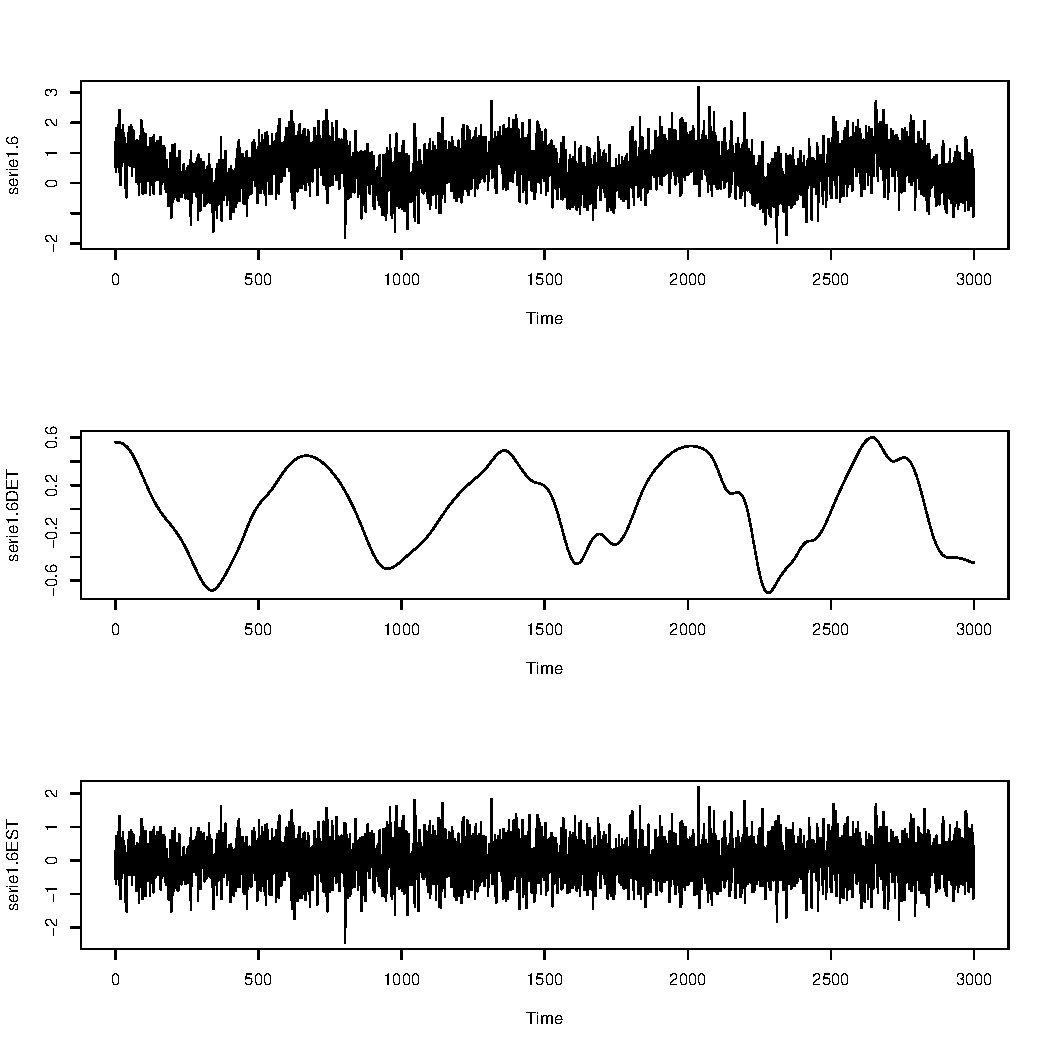
\includegraphics[scale=0.43]{serie1_6.pdf}
  \caption{Série 1.5 e Série 1.6}

\end{center}
\end{figure}

\graphicspath{{imagens/}}
\begin{figure}[H]
\begin{center}
  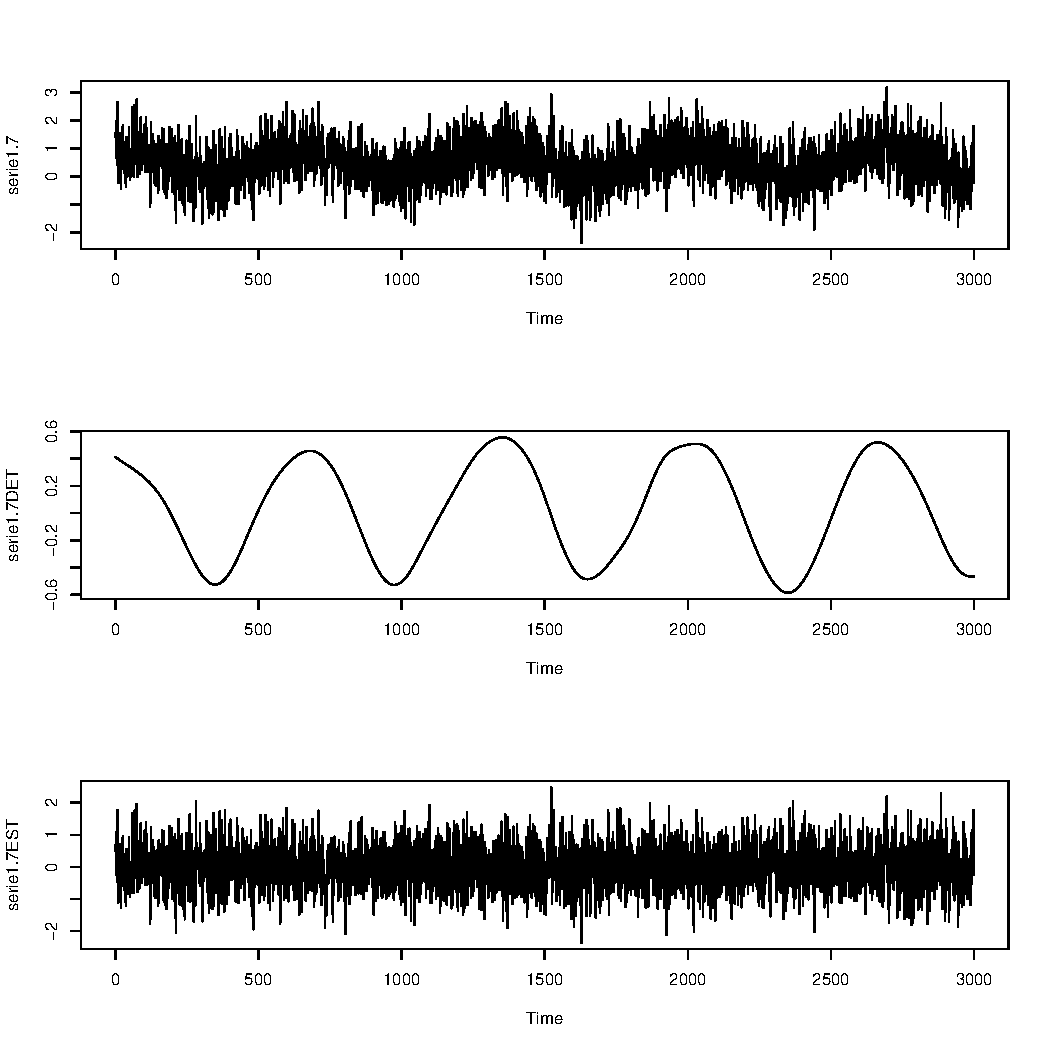
\includegraphics[scale=0.43]{serie1_7.pdf} \quad
  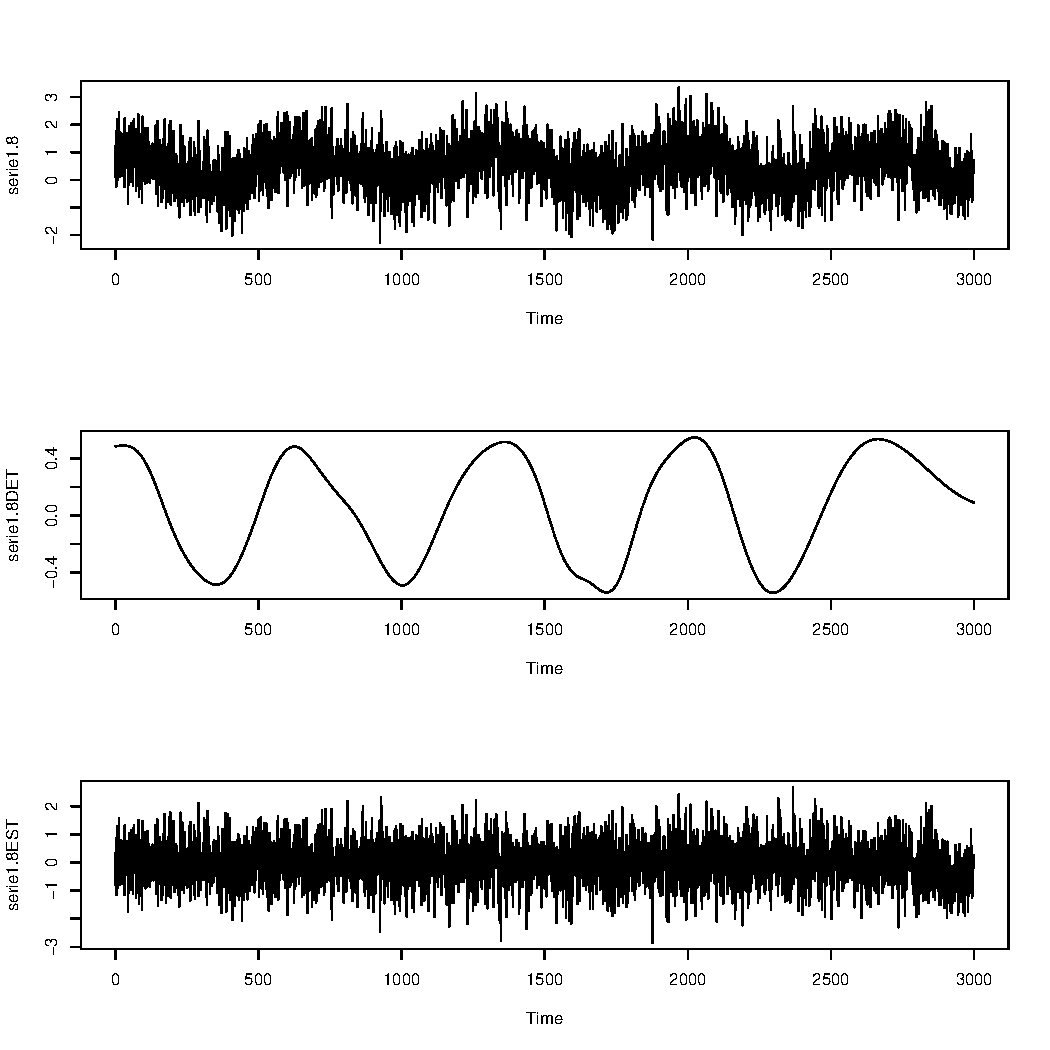
\includegraphics[scale=0.43]{serie1_8.pdf}
  \caption{Série 1.7 e Série 1.8}

\end{center}
\end{figure}

\graphicspath{{imagens/}}
\begin{figure}[H]
\begin{center}
  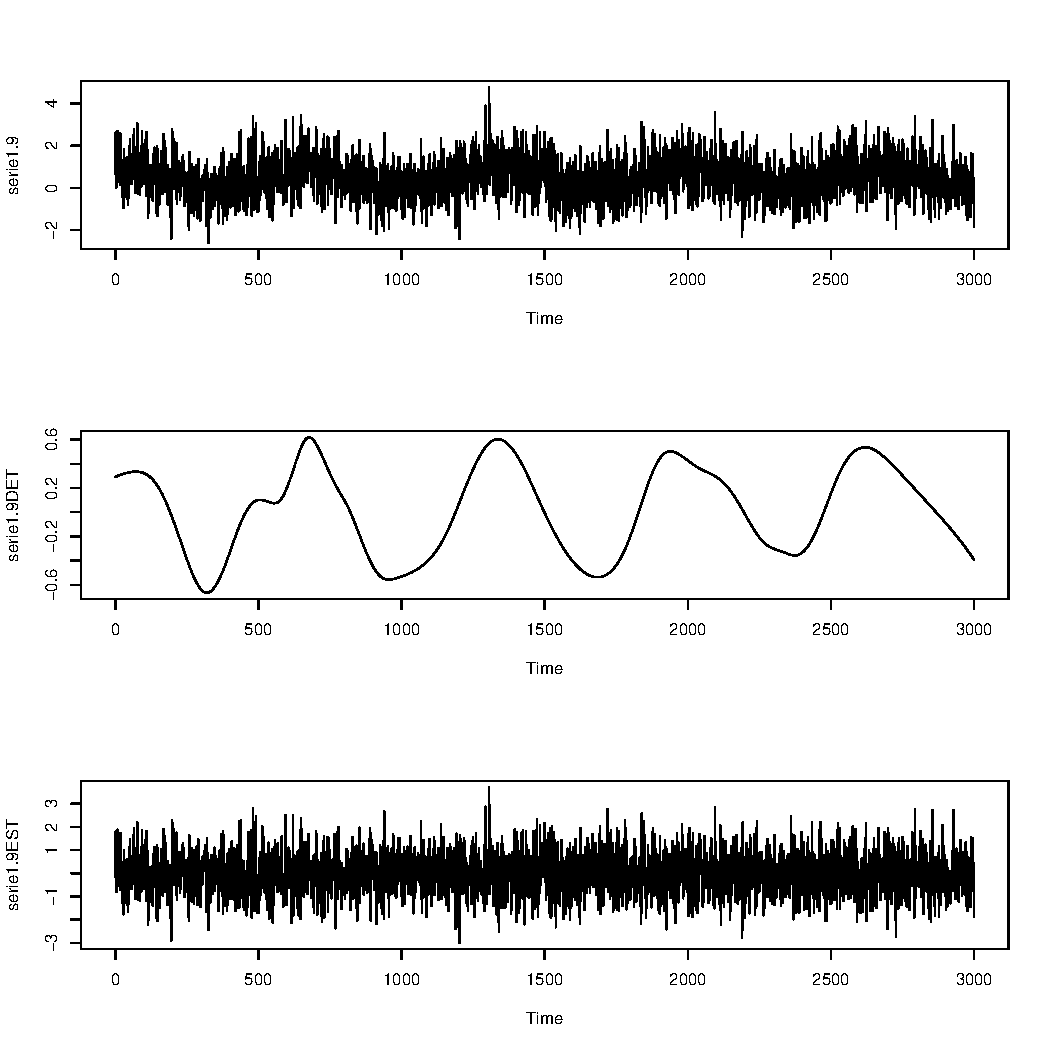
\includegraphics[scale=0.43]{serie1_9.pdf} \quad
  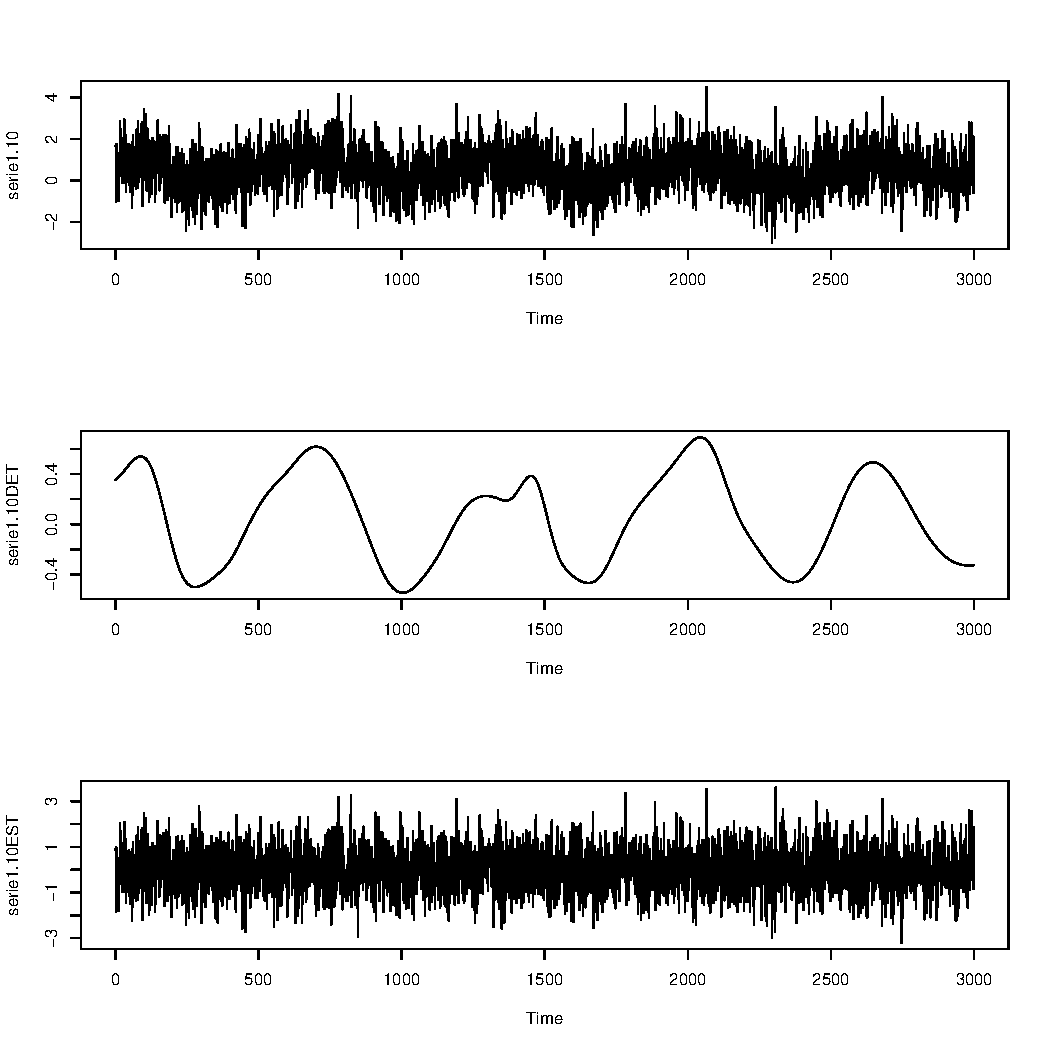
\includegraphics[scale=0.43]{serie1_10.pdf}
  \caption{Série 1.9 e Série 1.10}

\end{center}
\end{figure}

\section{Séries TIPO 2}
10 séries cossenoide com ruído ao longo da série e tendência.
\graphicspath{{imagens/}}
\begin{figure}[H]
\begin{center}
  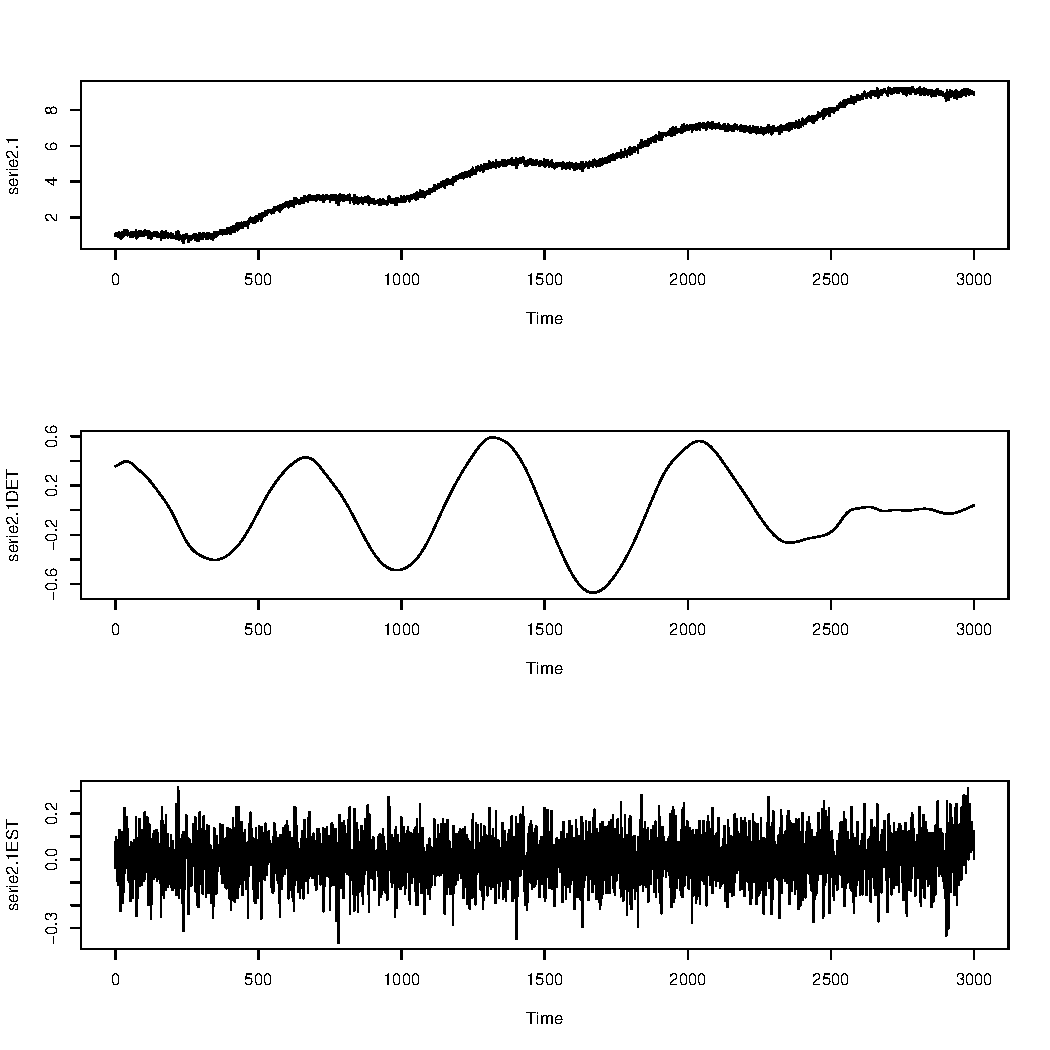
\includegraphics[scale=0.43]{serie2_1.pdf} \quad
  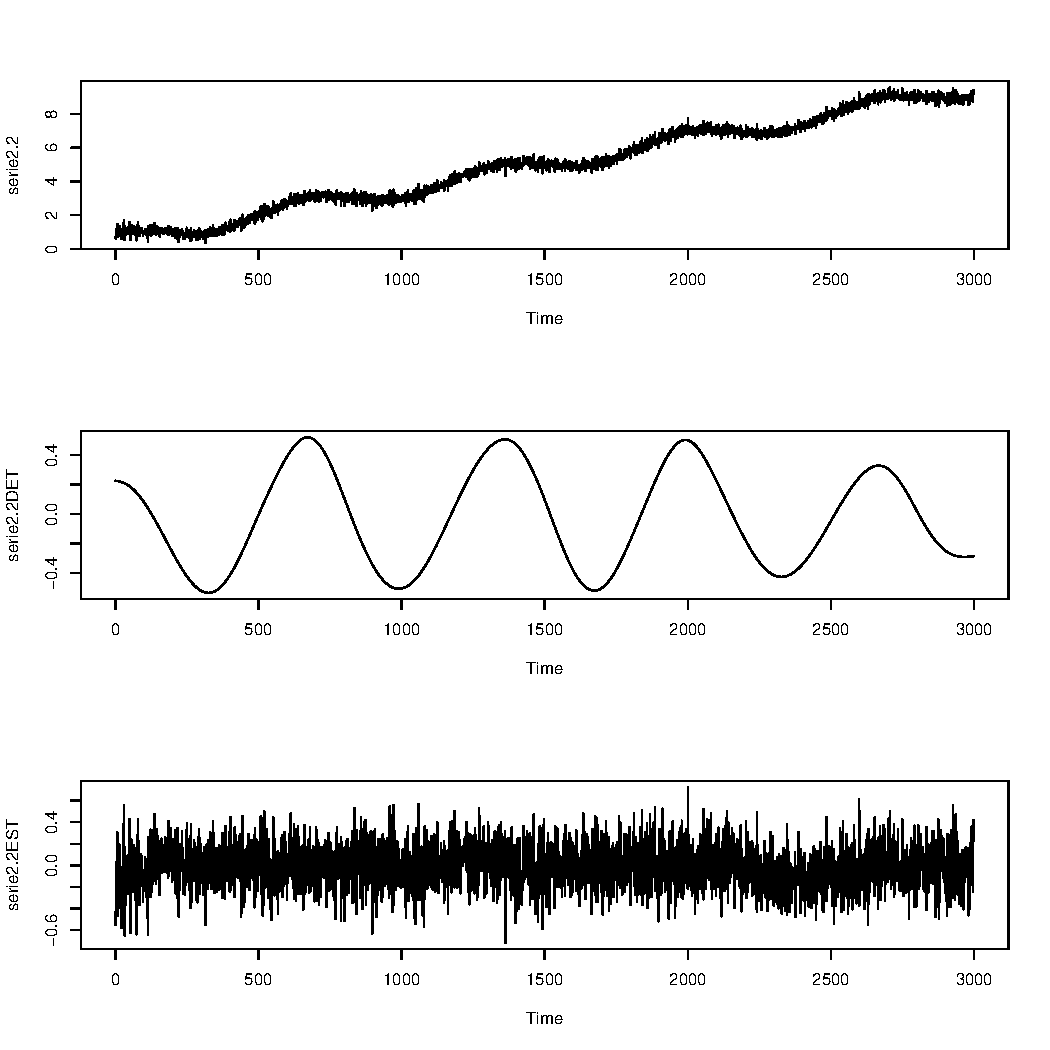
\includegraphics[scale=0.43]{serie2_2.pdf}
  \caption{Série 2.1 e Série 2.2}

\end{center}
\end{figure}

\graphicspath{{imagens/}}
\begin{figure}[H]
\begin{center}
  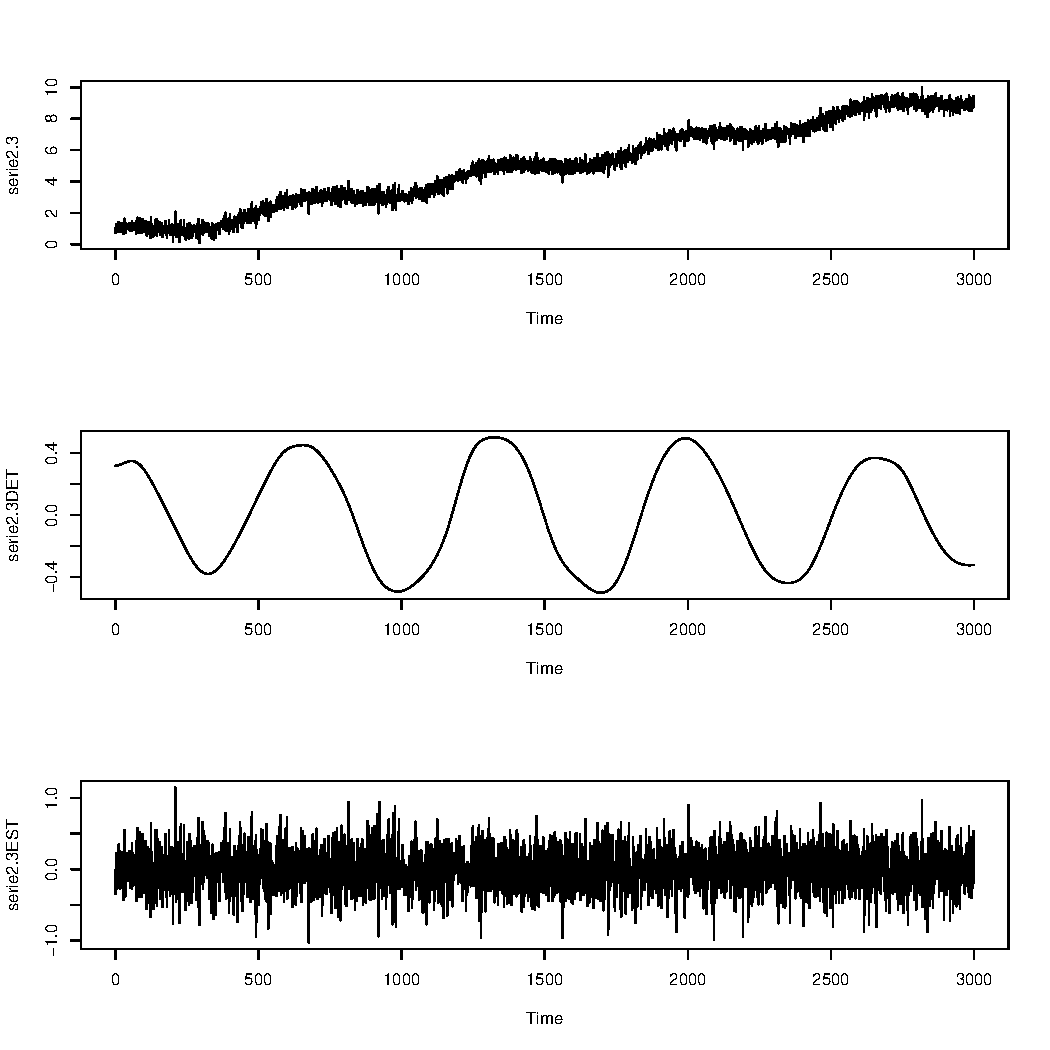
\includegraphics[scale=0.43]{serie2_3.pdf} \quad
  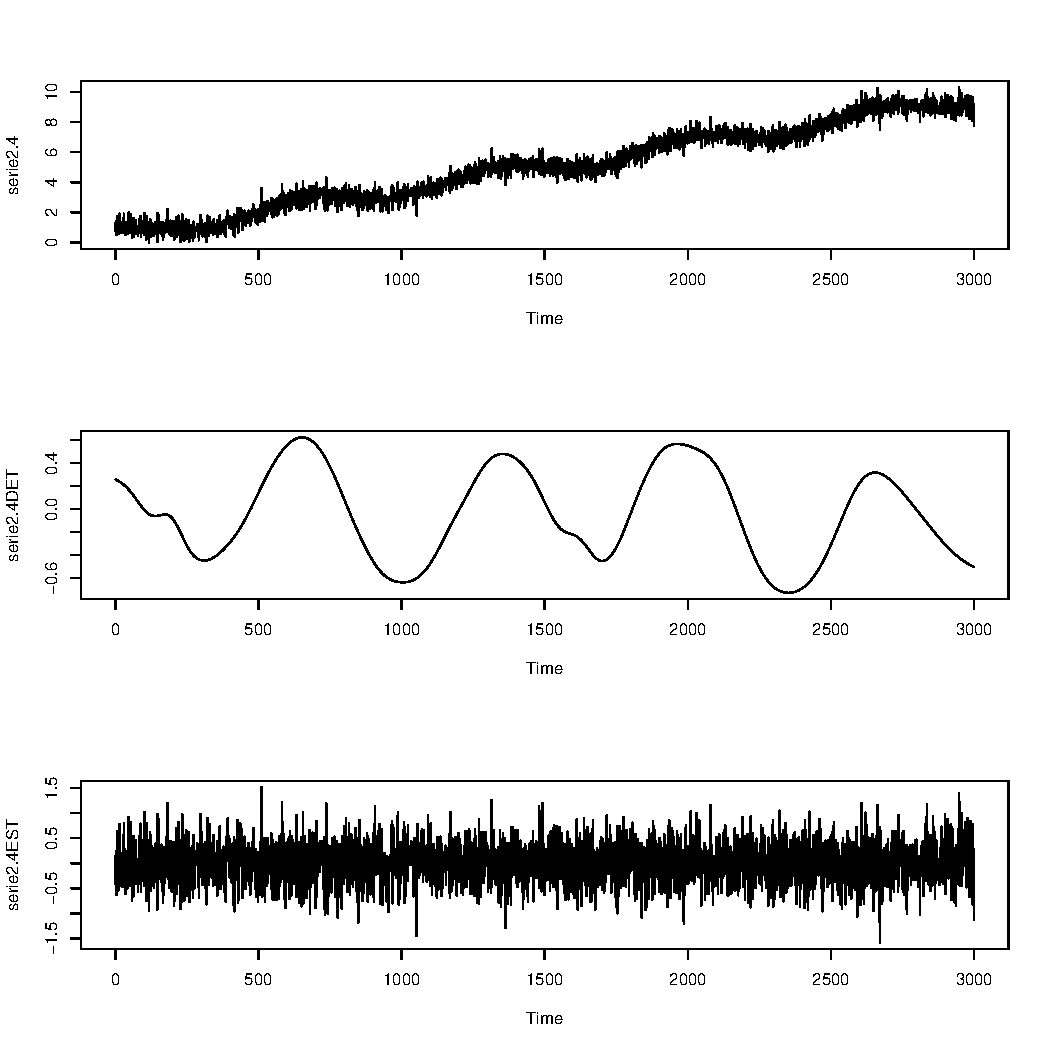
\includegraphics[scale=0.43]{serie2_4.pdf}
  \caption{Série 2.3 e Série 2.4}

\end{center}
\end{figure}

\graphicspath{{imagens/}}
\begin{figure}[H]
\begin{center}
  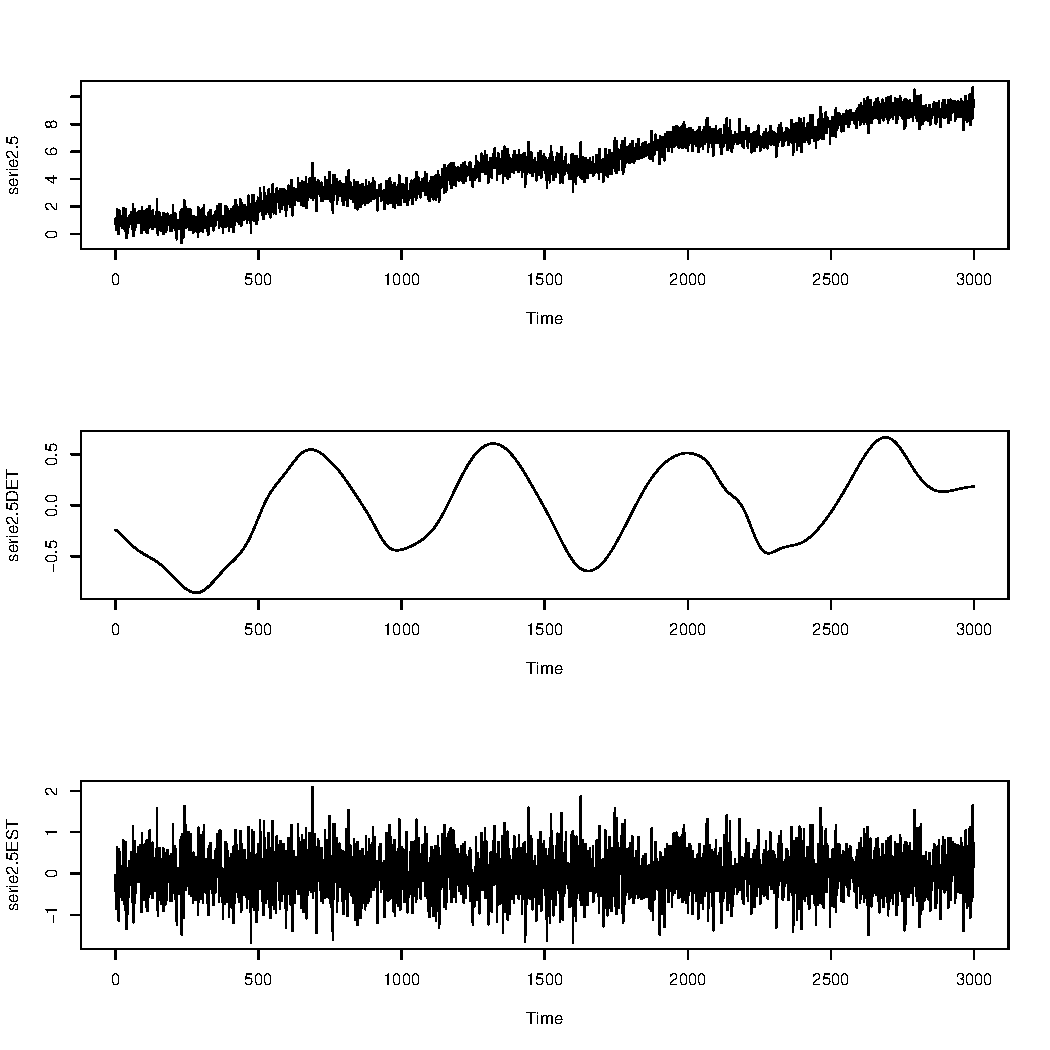
\includegraphics[scale=0.43]{serie2_5.pdf} \quad
  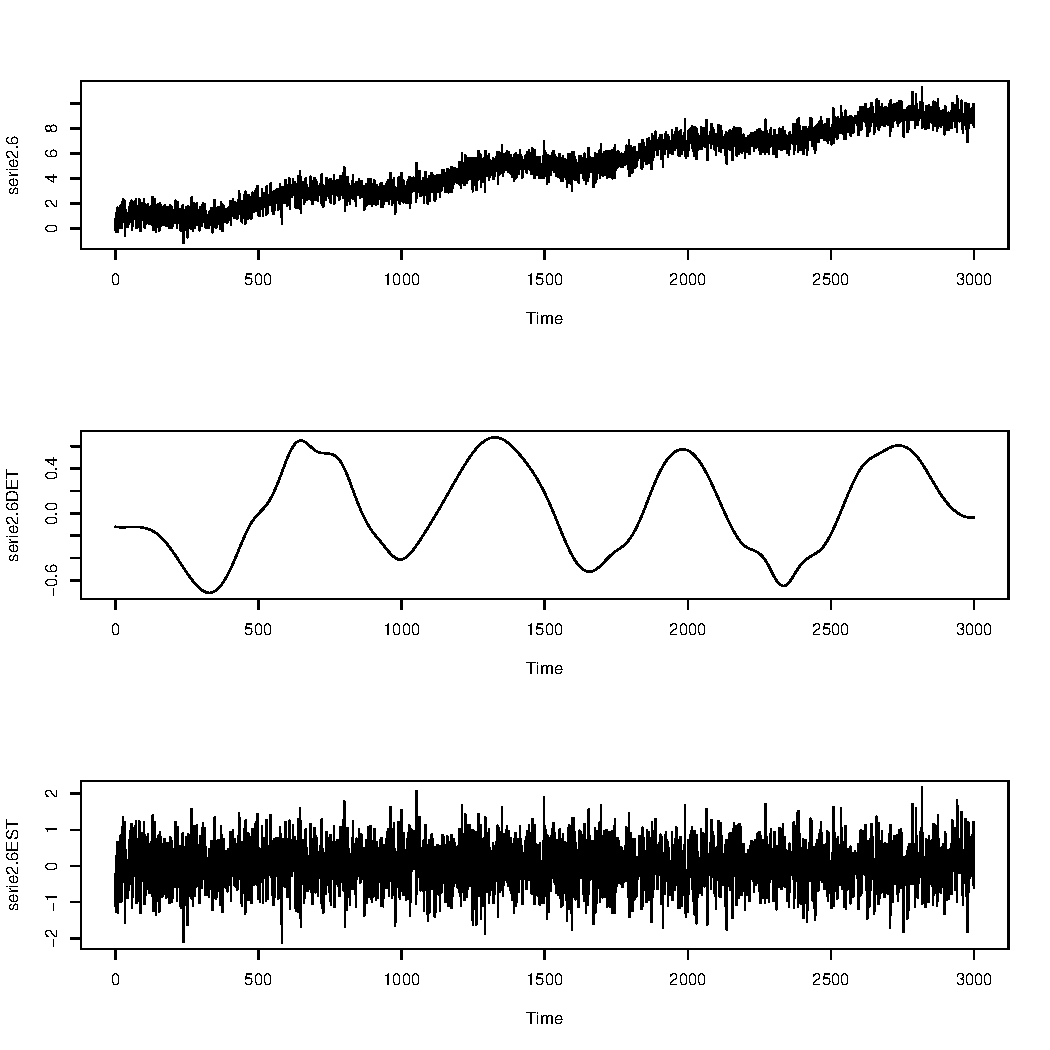
\includegraphics[scale=0.43]{serie2_6.pdf}
  \caption{Série 2.5 e Série 2.6}

\end{center}
\end{figure}

\graphicspath{{imagens/}}
\begin{figure}[H]
\begin{center}
  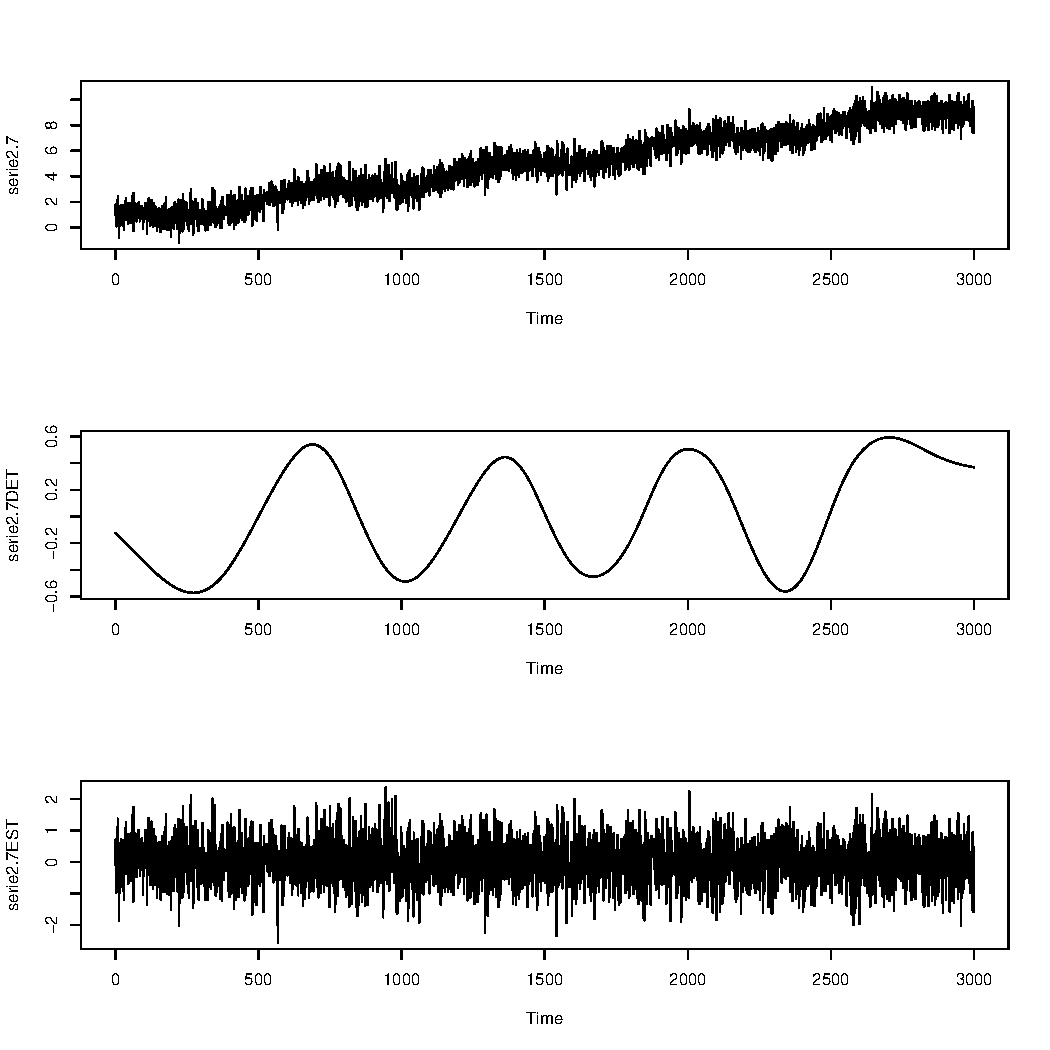
\includegraphics[scale=0.43]{serie2_7.pdf} \quad
  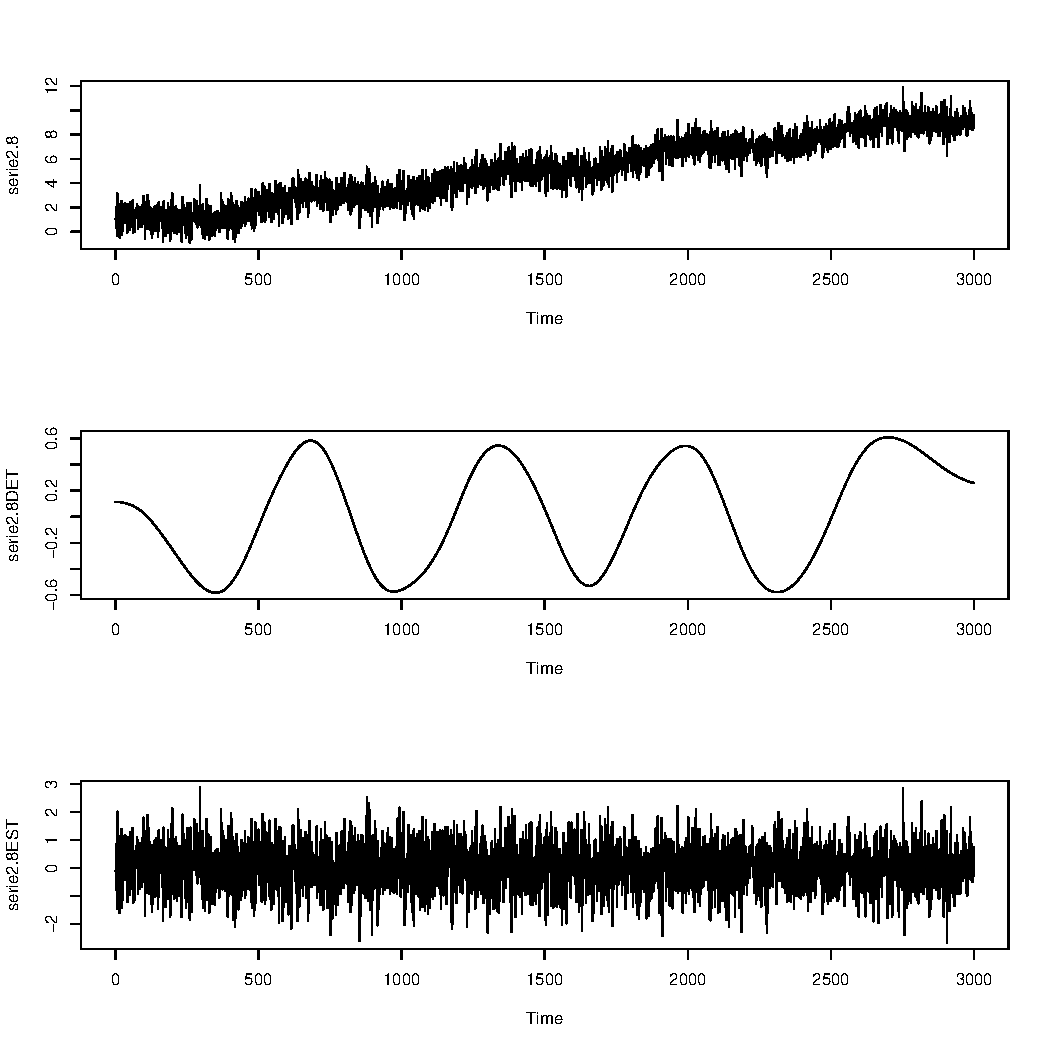
\includegraphics[scale=0.43]{serie2_8.pdf}
  \caption{Série 2.7 e Série 2.8}

\end{center}
\end{figure}

\graphicspath{{imagens/}}
\begin{figure}[H]
\begin{center}
  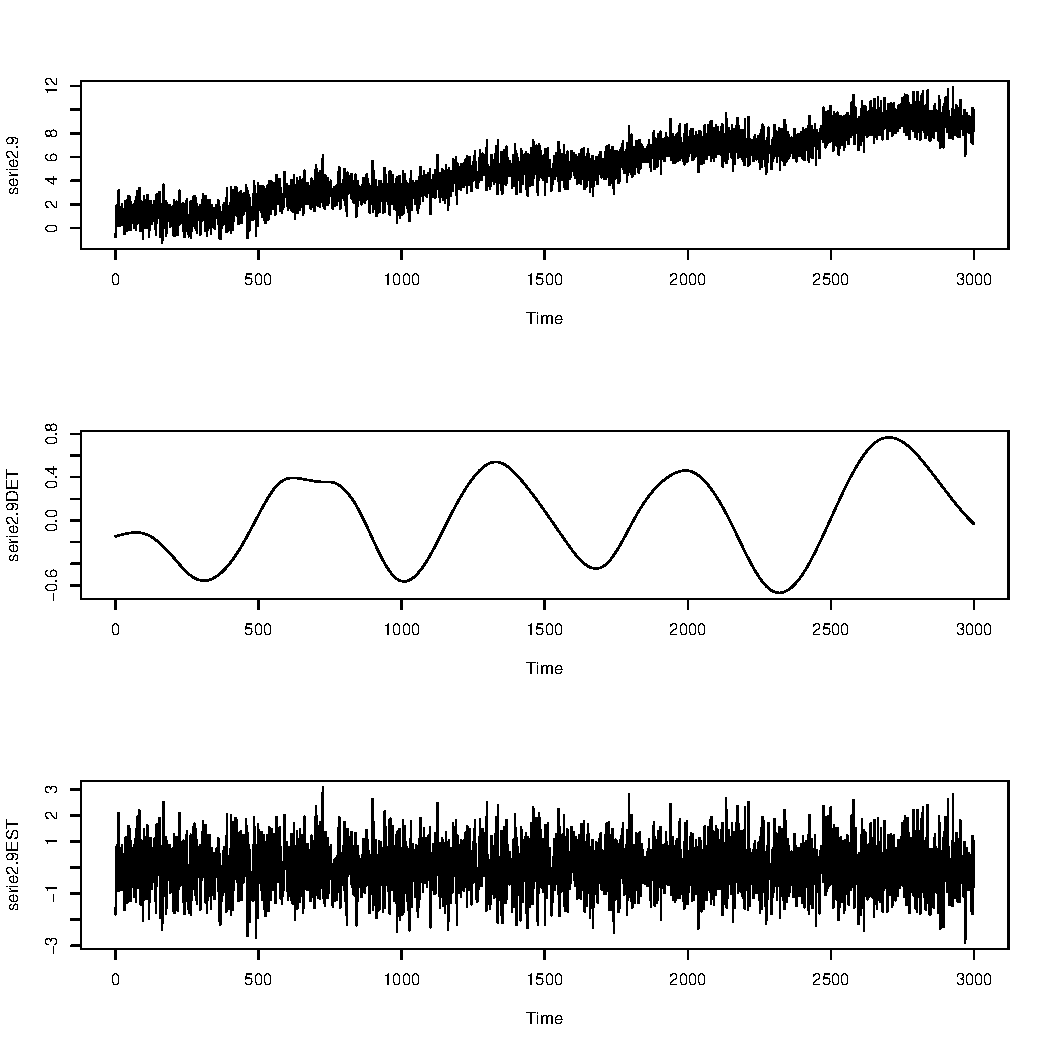
\includegraphics[scale=0.43]{serie2_9.pdf} \quad
  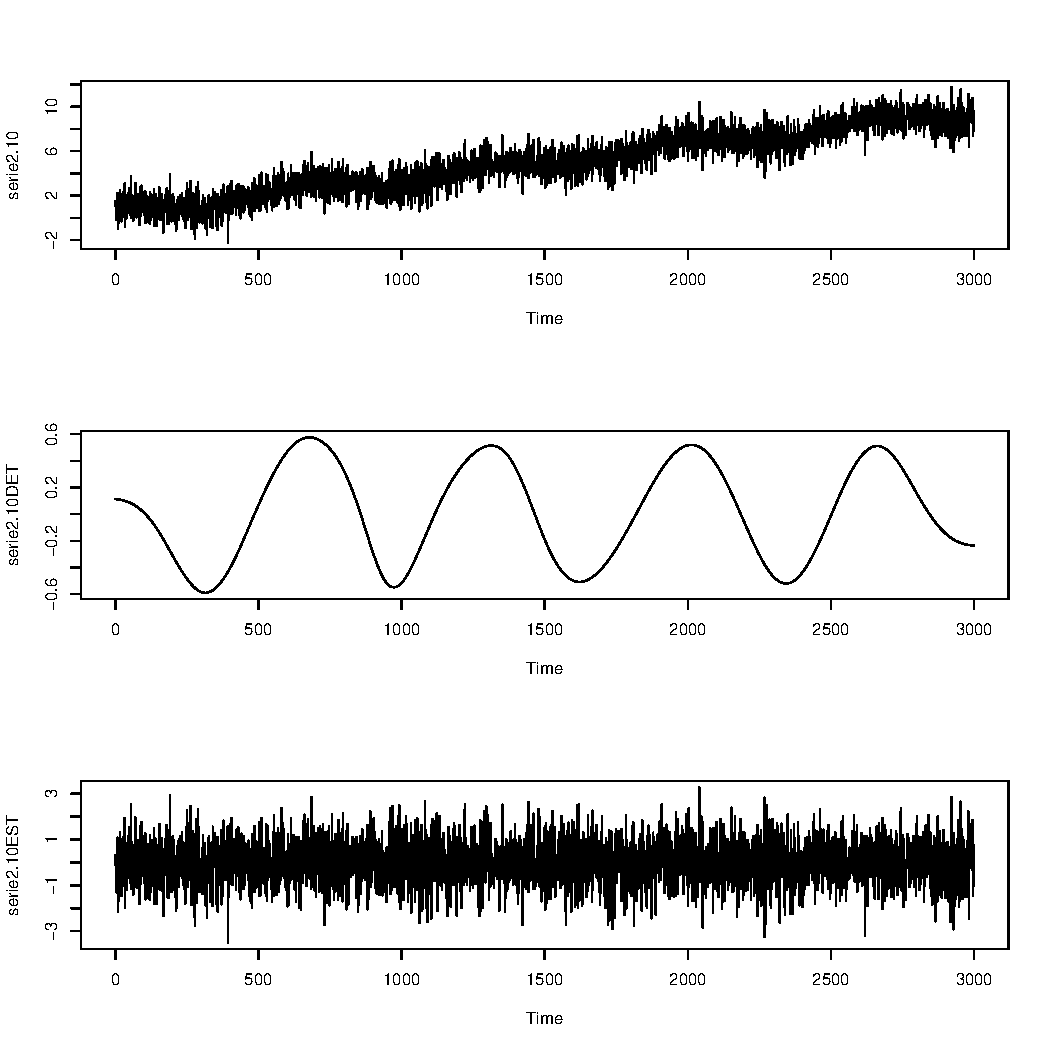
\includegraphics[scale=0.43]{serie2_10.pdf}
  \caption{Série 2.9 e Série 2.10}

\end{center}
\end{figure}

\section{Séries TIPO 3}
10 séries senoide com ruído ao longo da série.
\graphicspath{{imagens/}}
\begin{figure}[H]
\begin{center}
  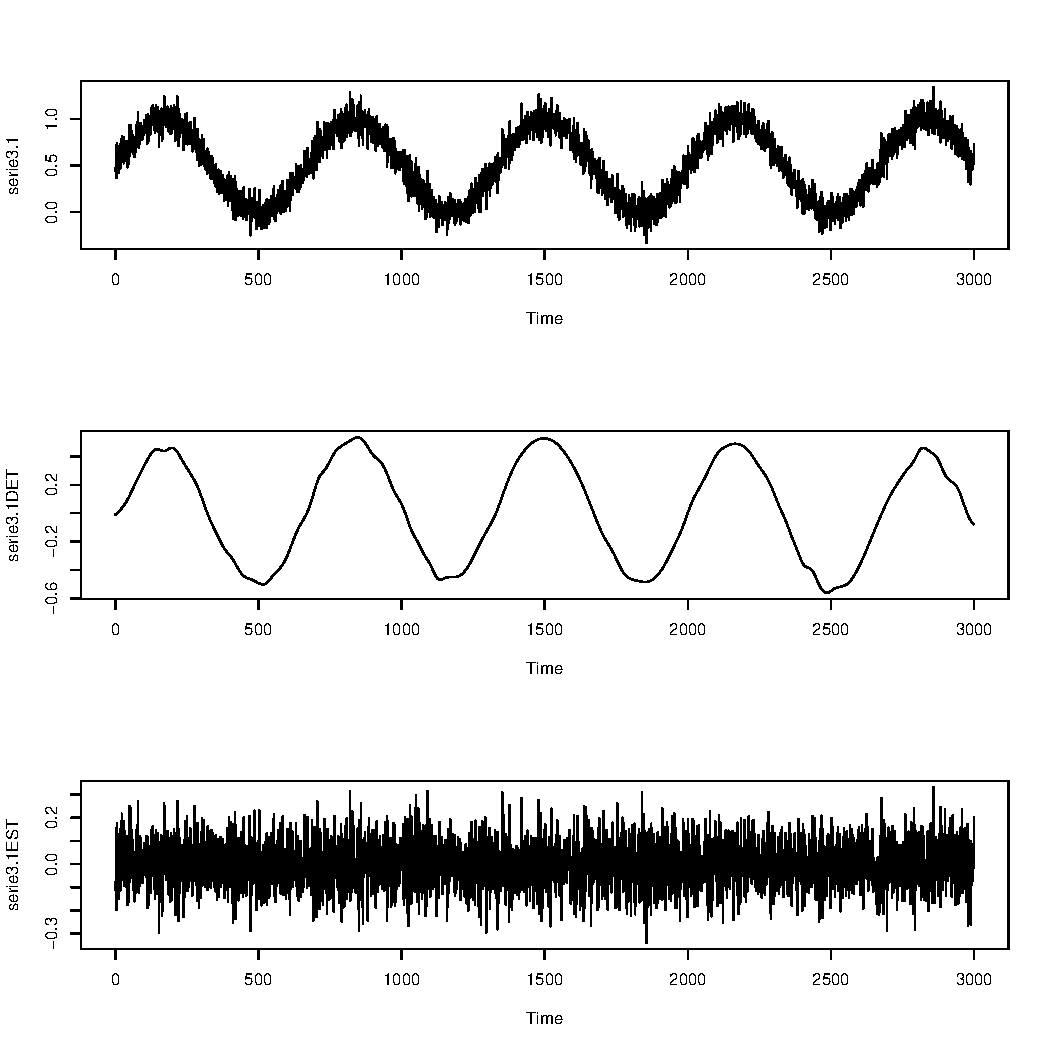
\includegraphics[scale=0.43]{serie3_1.pdf} \quad
  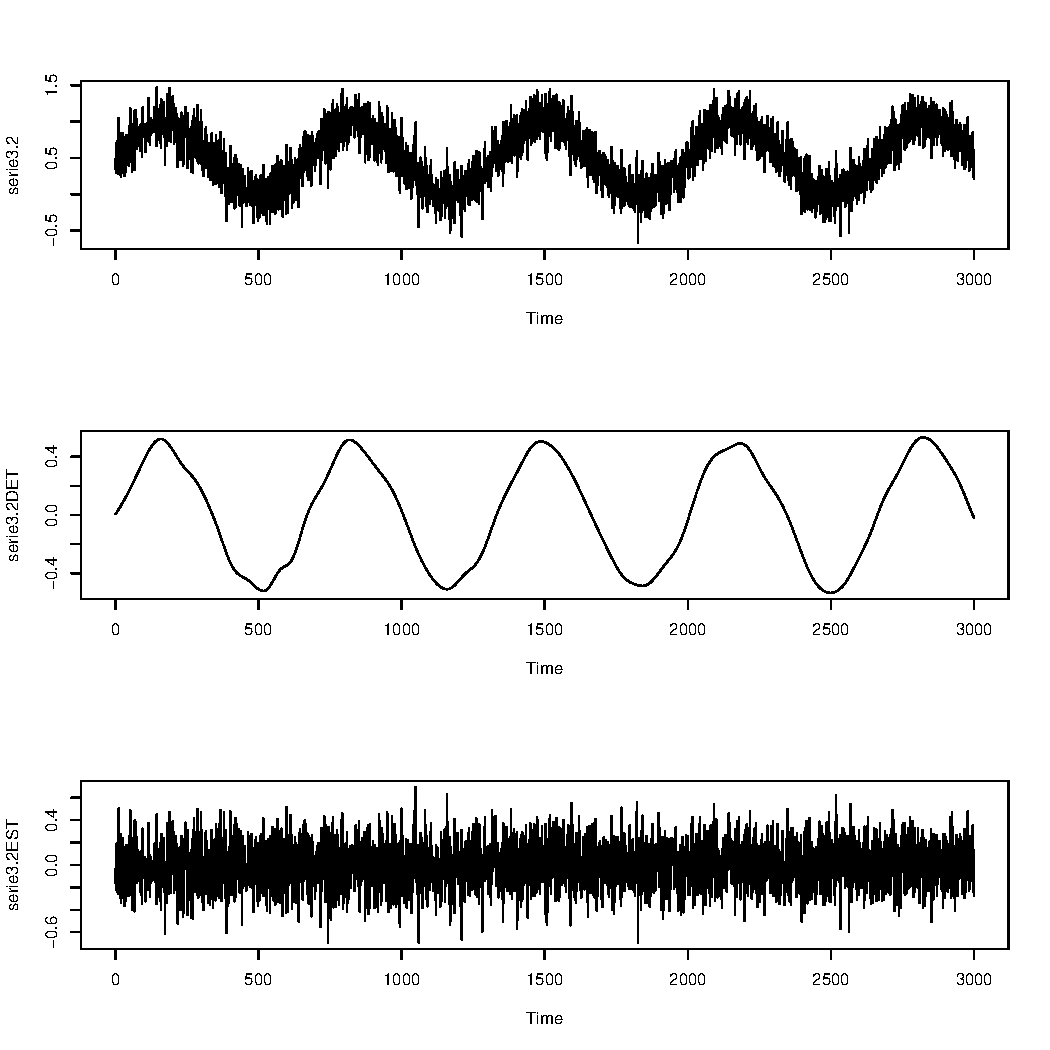
\includegraphics[scale=0.43]{serie3_2.pdf}
  \caption{Série 3.1 e Série 3.2}

\end{center}
\end{figure}

\graphicspath{{imagens/}}
\begin{figure}[H]
\begin{center}
  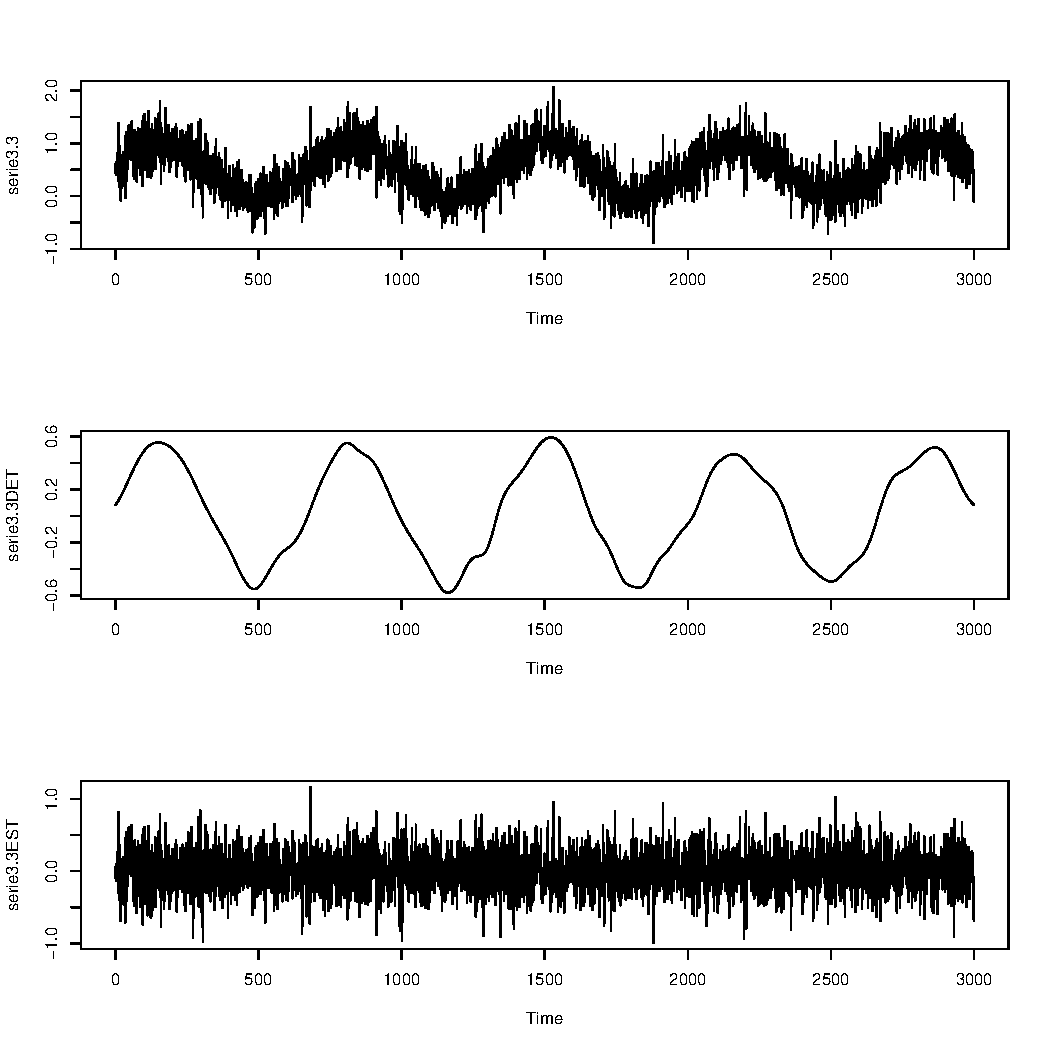
\includegraphics[scale=0.43]{serie3_3.pdf} \quad
  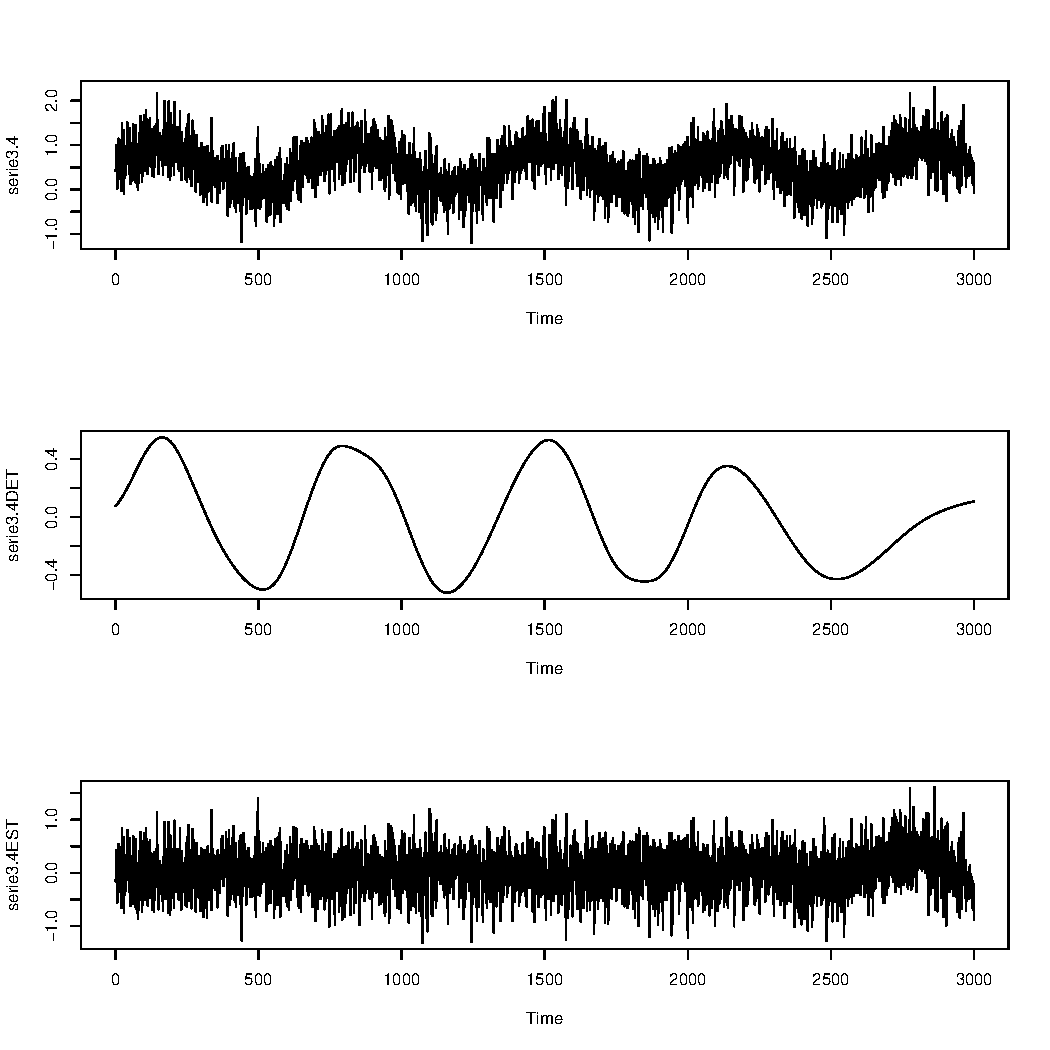
\includegraphics[scale=0.43]{serie3_4.pdf}
  \caption{Série 3.3 e Série 3.4}

\end{center}
\end{figure}

\graphicspath{{imagens/}}
\begin{figure}[H]
\begin{center}
  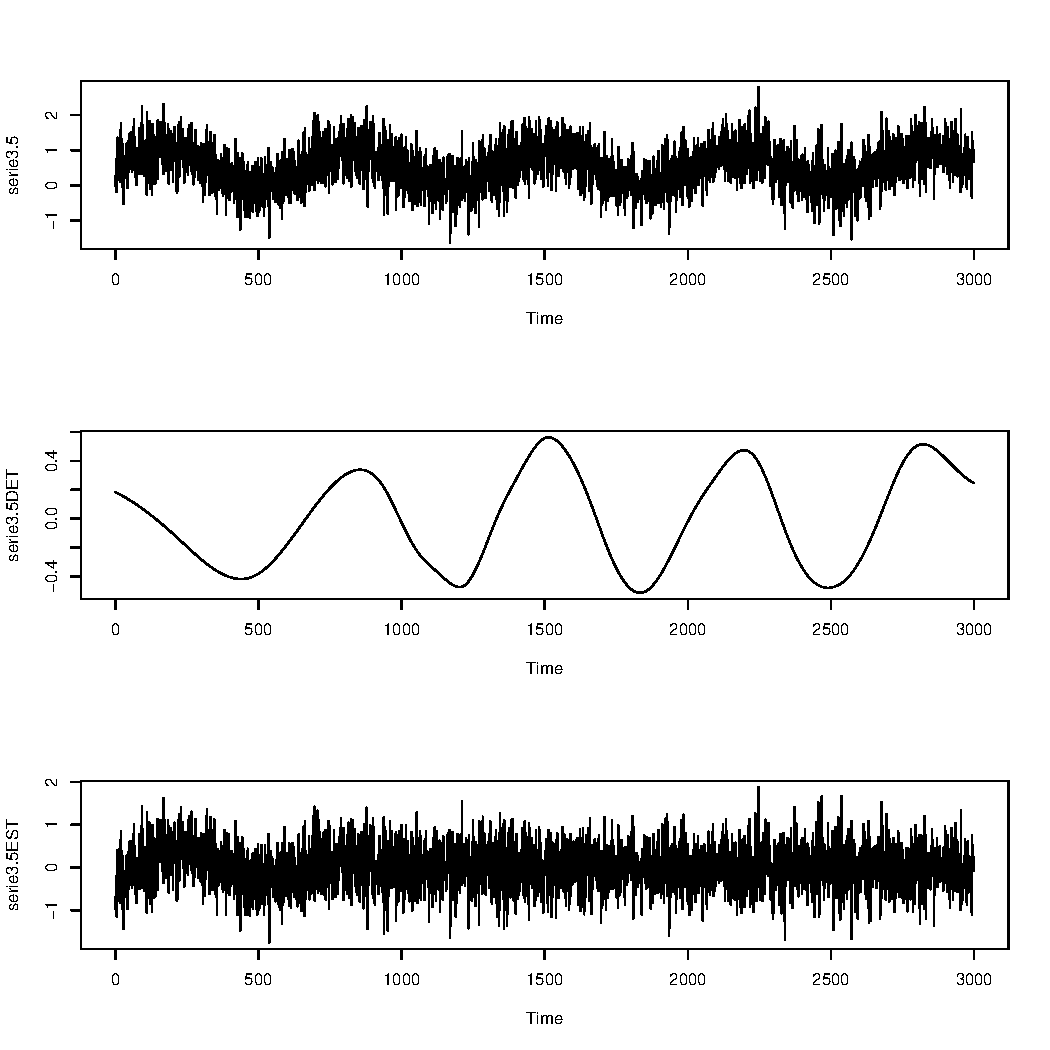
\includegraphics[scale=0.43]{serie3_5.pdf} \quad
  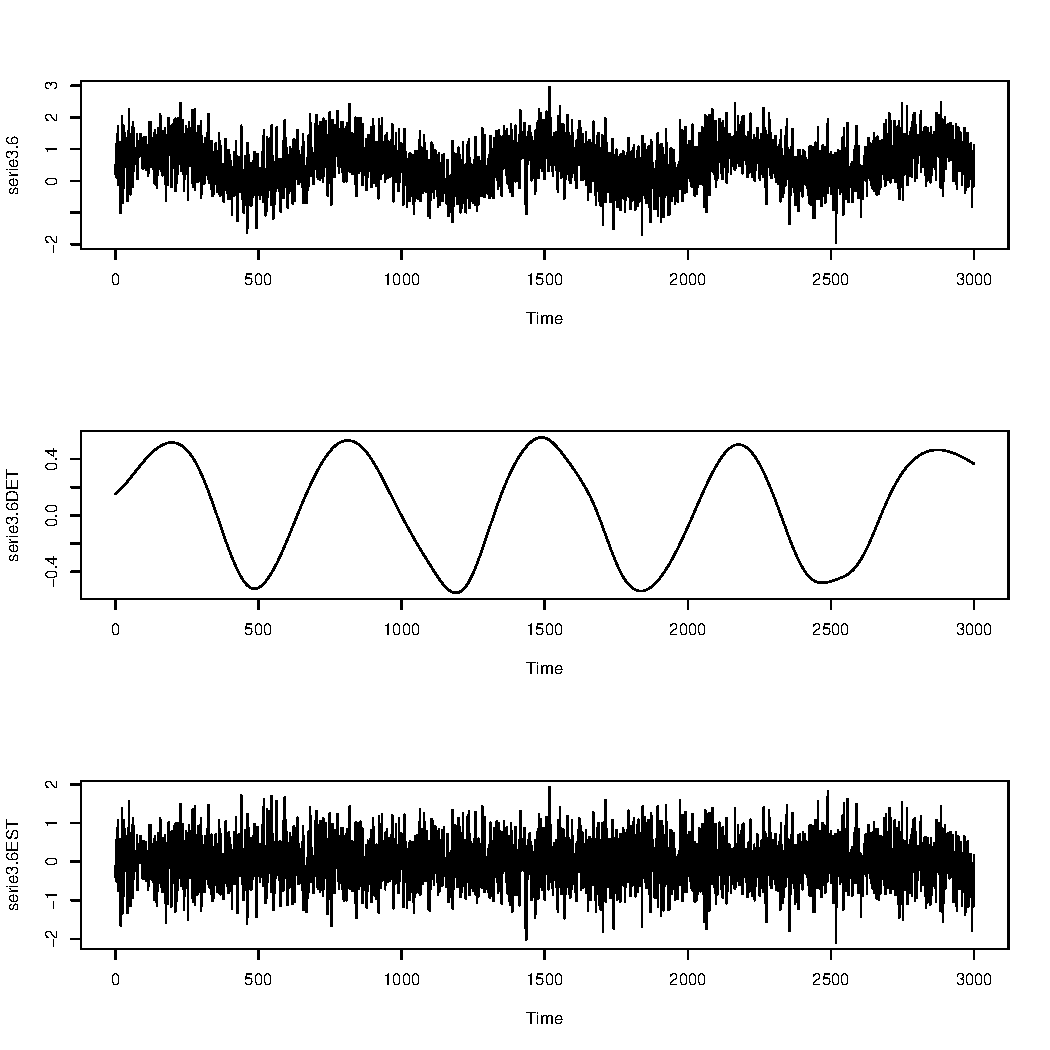
\includegraphics[scale=0.43]{serie3_6.pdf}
  \caption{Série 3.5 e Série 3.6}

\end{center}
\end{figure}

\graphicspath{{imagens/}}
\begin{figure}[H]
\begin{center}
  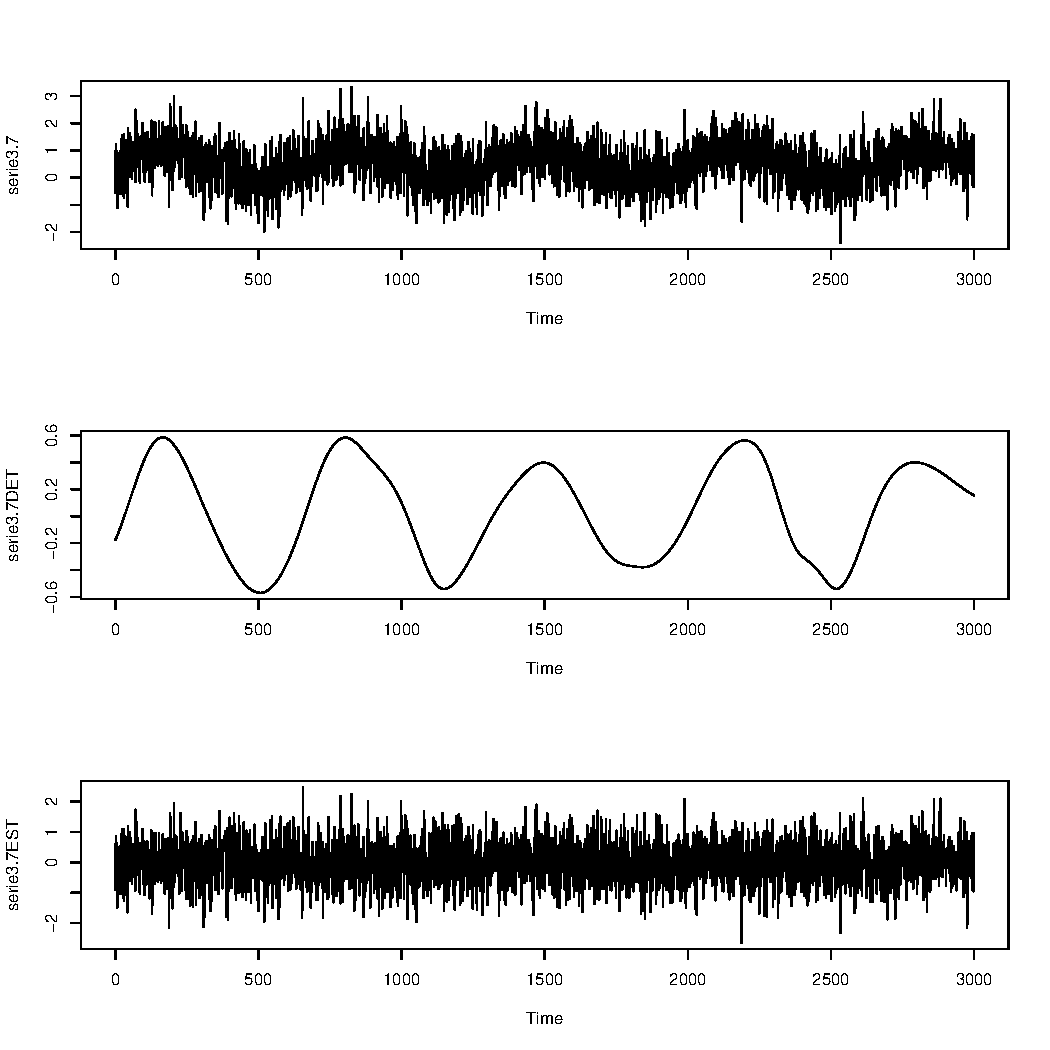
\includegraphics[scale=0.43]{serie3_7.pdf} \quad
  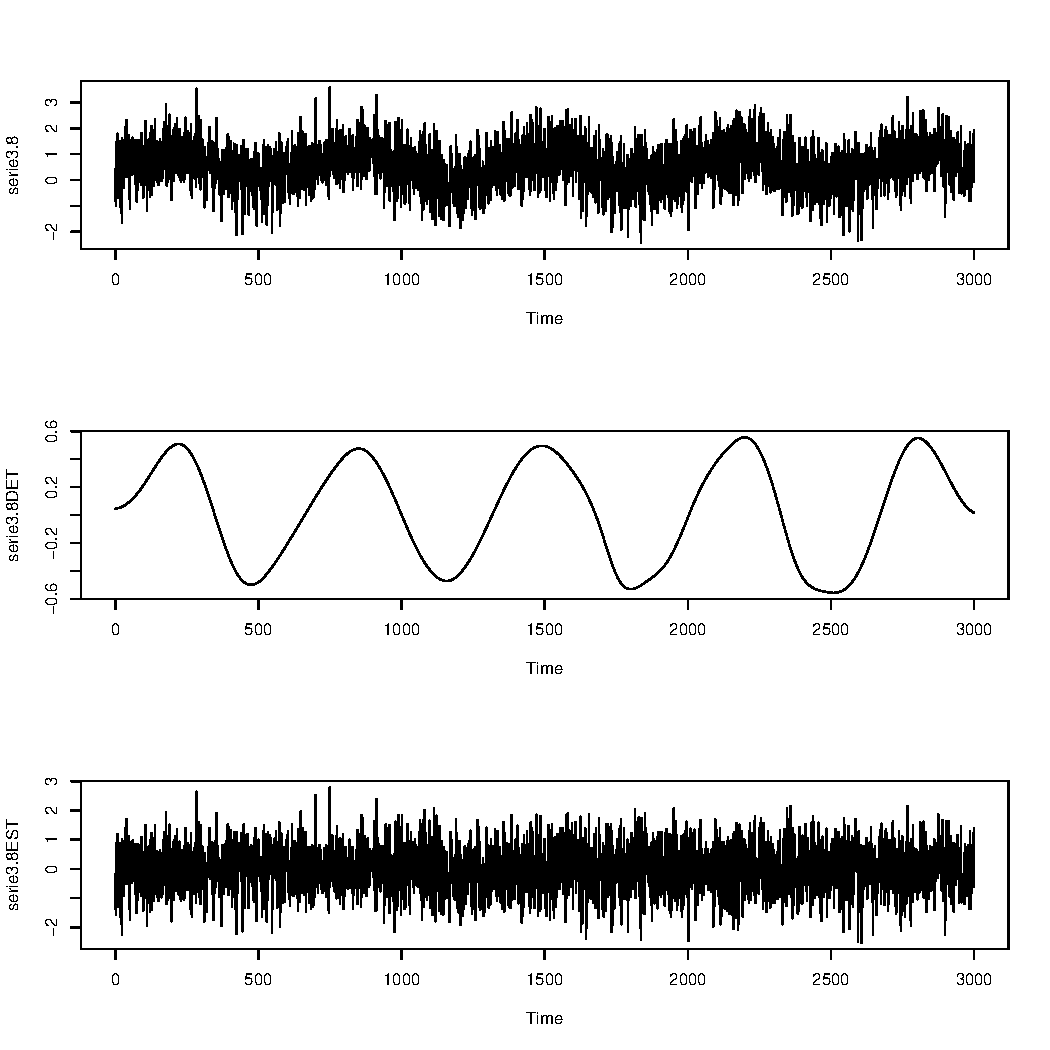
\includegraphics[scale=0.43]{serie3_8.pdf}
  \caption{Série 3.7 e Série 3.8}

\end{center}
\end{figure}

\graphicspath{{imagens/}}
\begin{figure}[H]
\begin{center}
  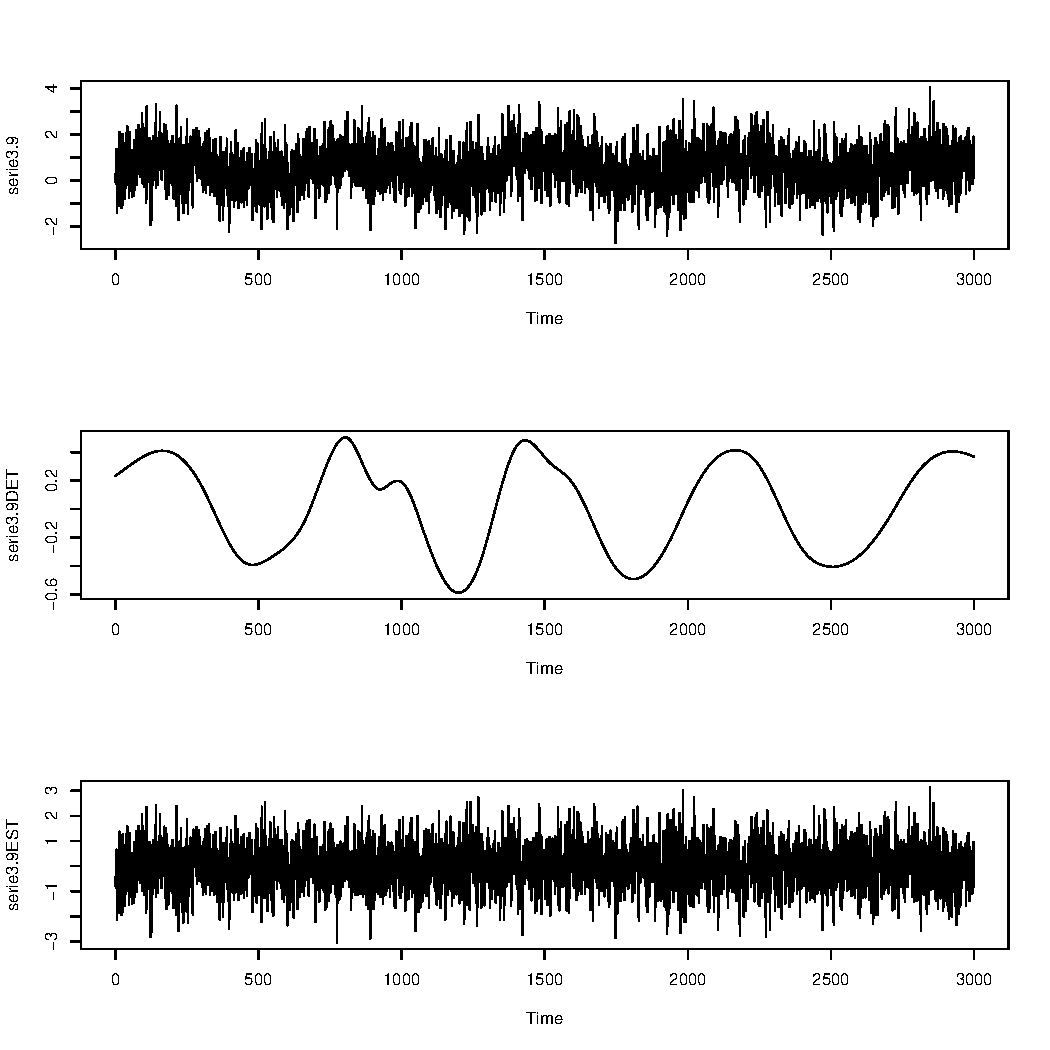
\includegraphics[scale=0.43]{serie3_9.pdf} \quad
  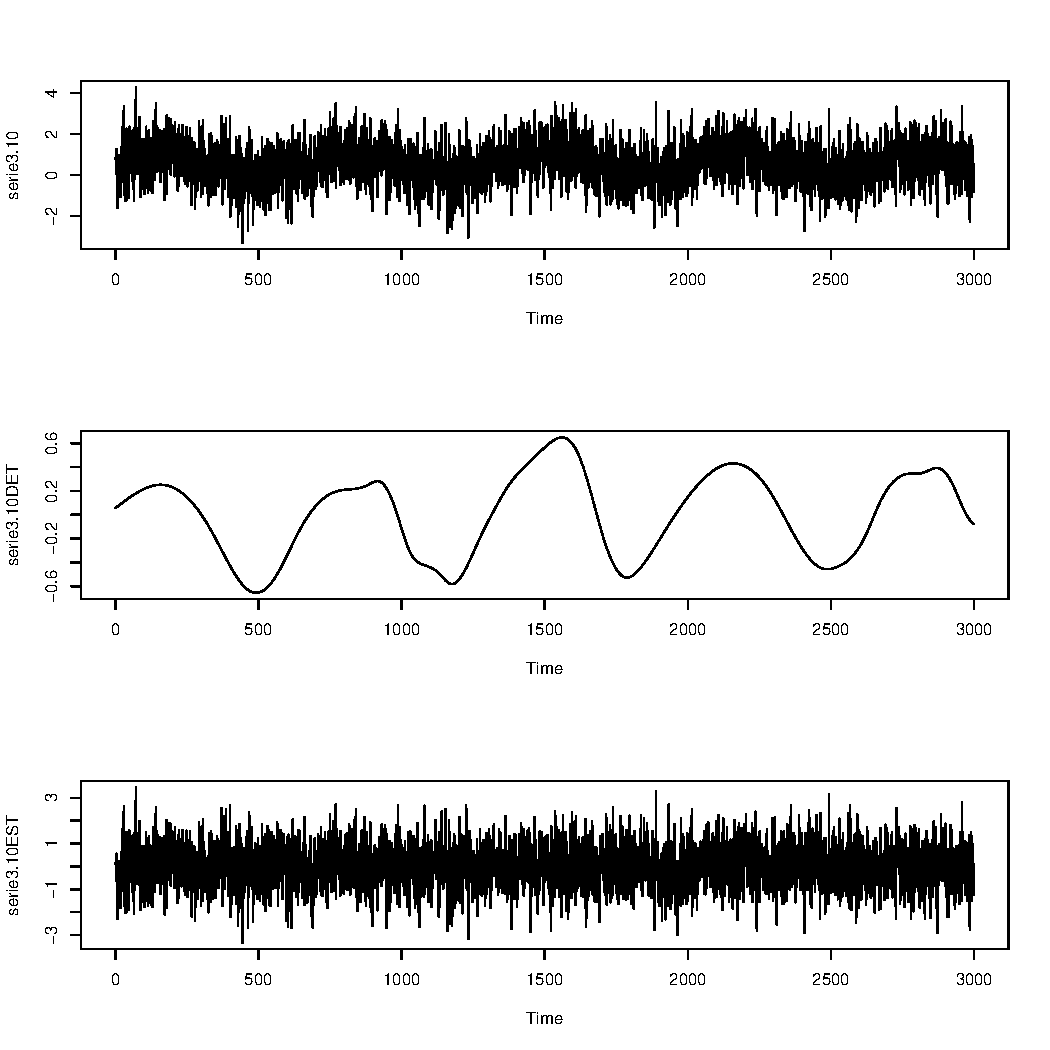
\includegraphics[scale=0.43]{serie3_10.pdf}
  \caption{Série 3.9 e Série 3.10}

\end{center}
\end{figure}

\section{Séries TIPO 4}
10 séries senoide com ruído ao longo da série e tendência.
\graphicspath{{imagens/}}
\begin{figure}[H]
\begin{center}
  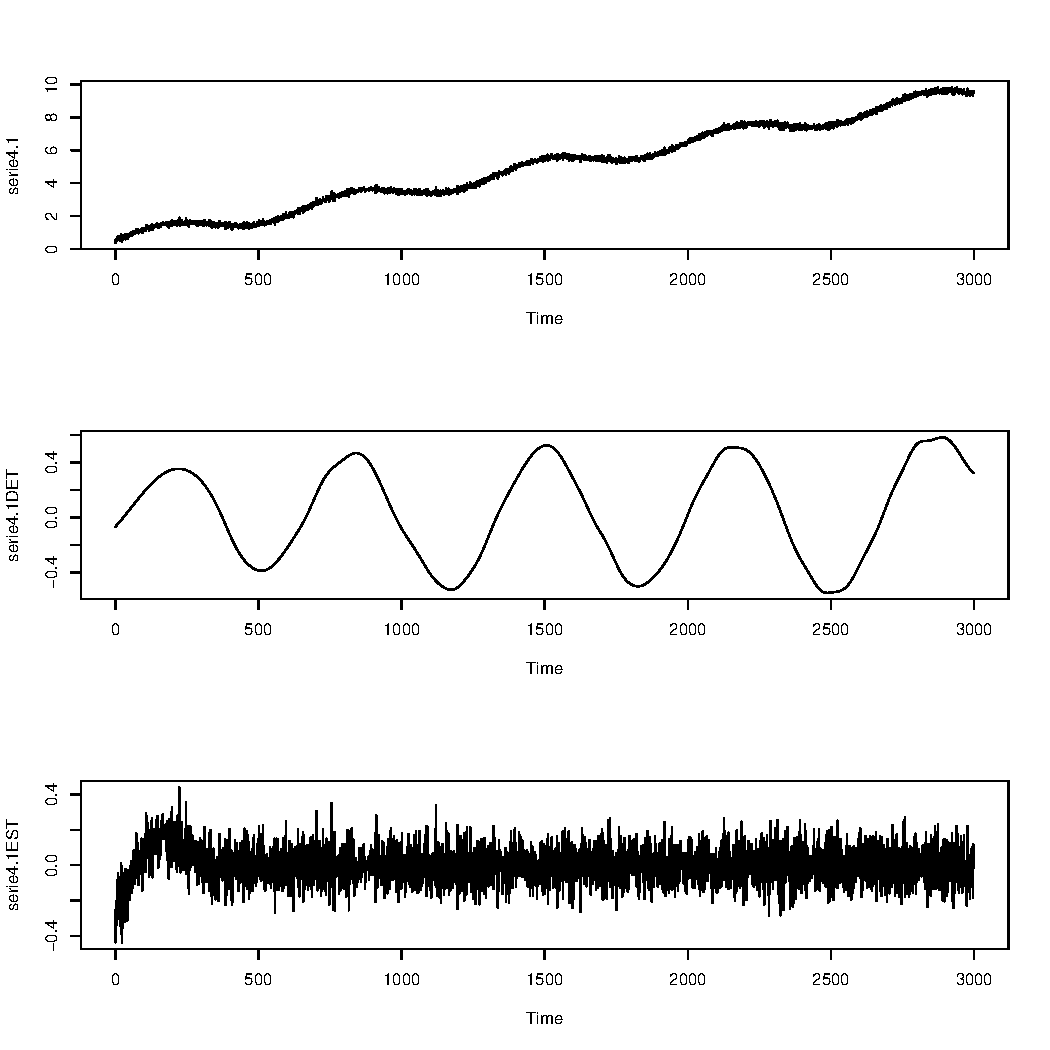
\includegraphics[scale=0.43]{serie4_1.pdf} \quad
  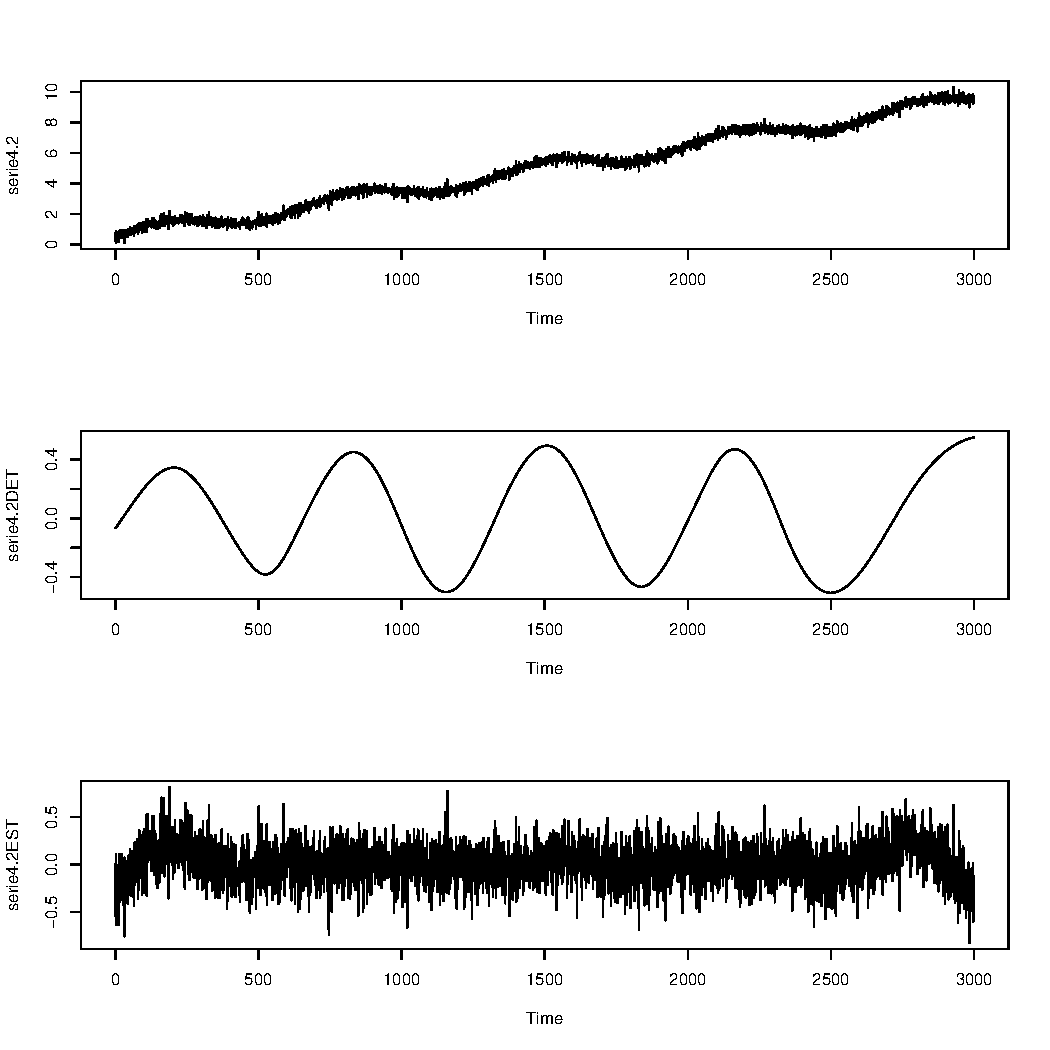
\includegraphics[scale=0.43]{serie4_2.pdf}
  \caption{Série 4.1 e Série 4.2}
\end{center}
\end{figure}

\graphicspath{{imagens/}}
\begin{figure}[H]
\begin{center}
  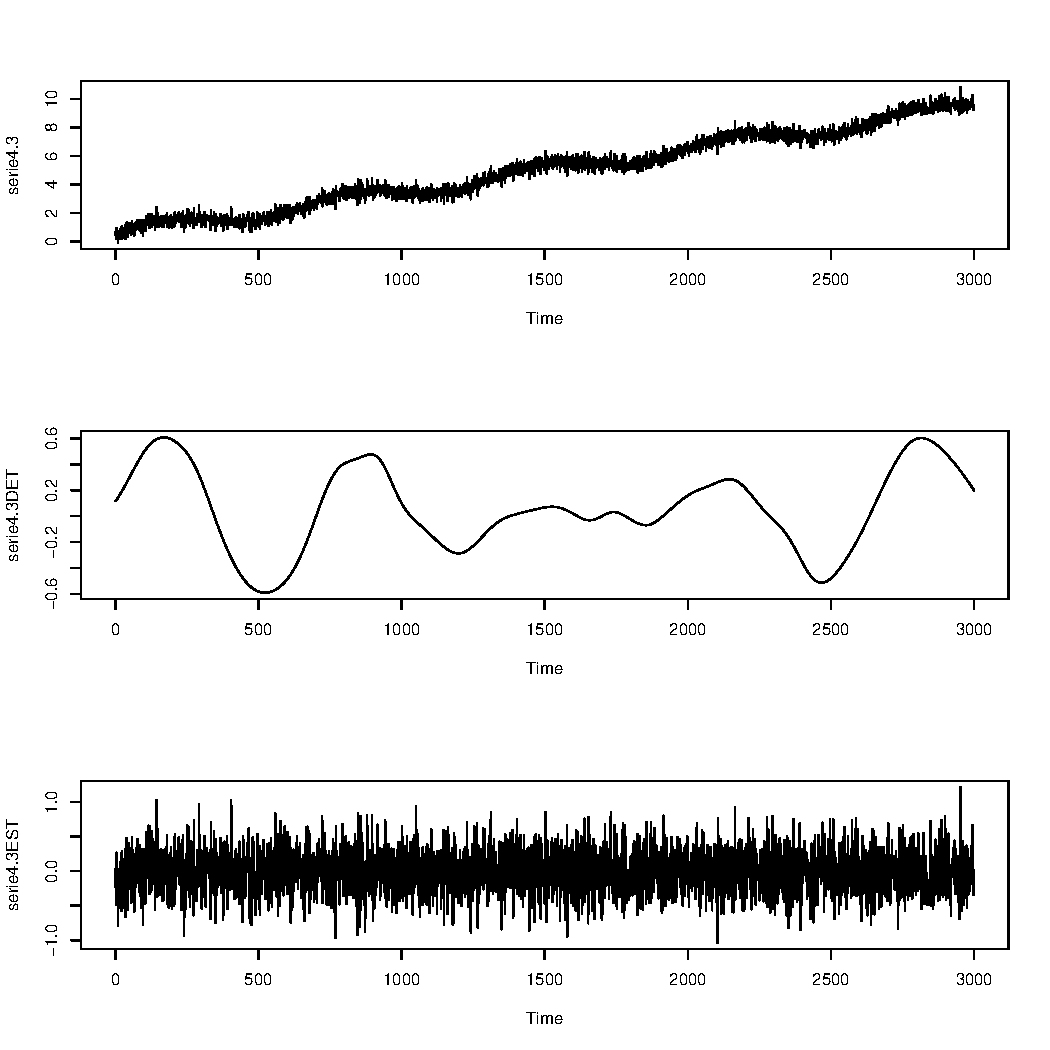
\includegraphics[scale=0.43]{serie4_3.pdf} \quad
 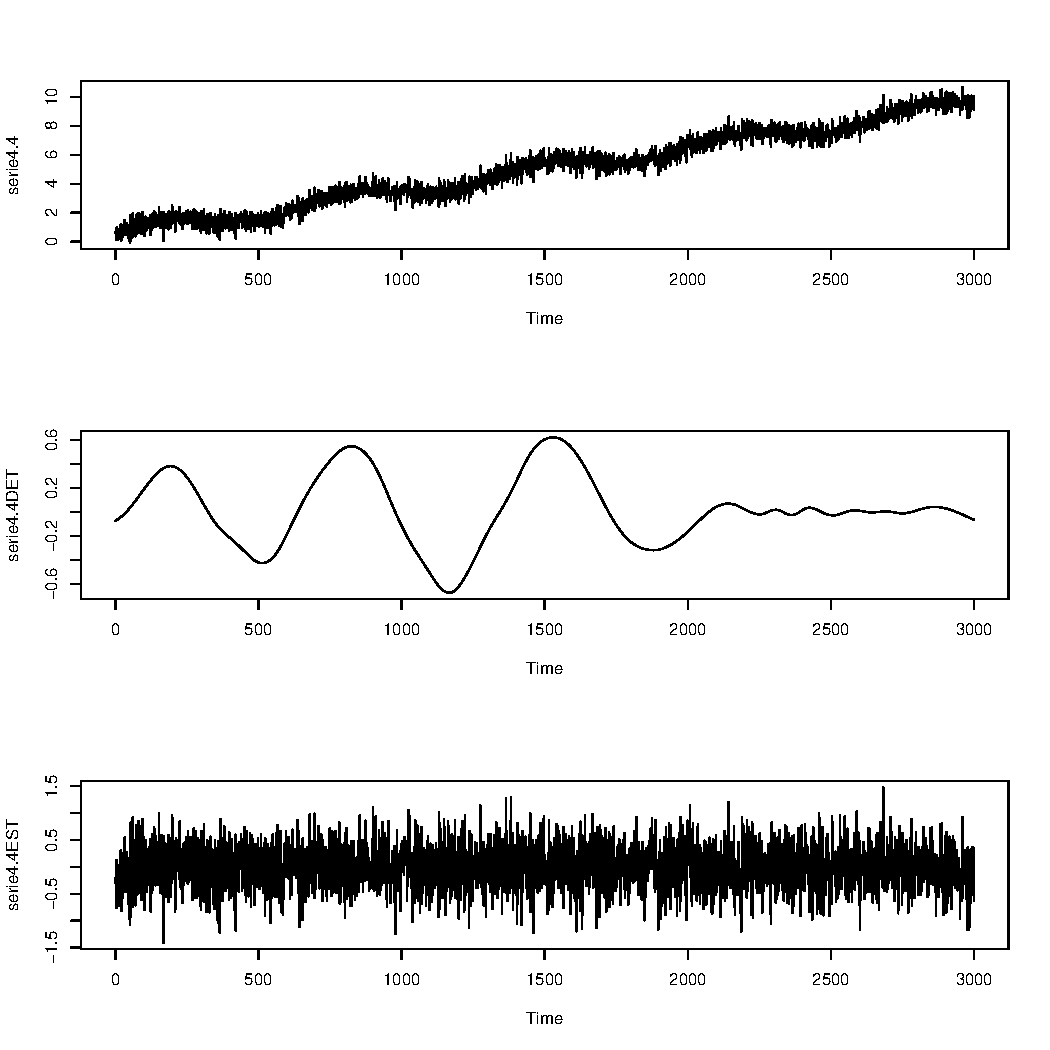
\includegraphics[scale=0.43]{serie4_4.pdf}
 \caption{Série 4.3 e Série 4.4}

\end{center}
\end{figure}

\graphicspath{{imagens/}}
\begin{figure}[H]
\begin{center}
  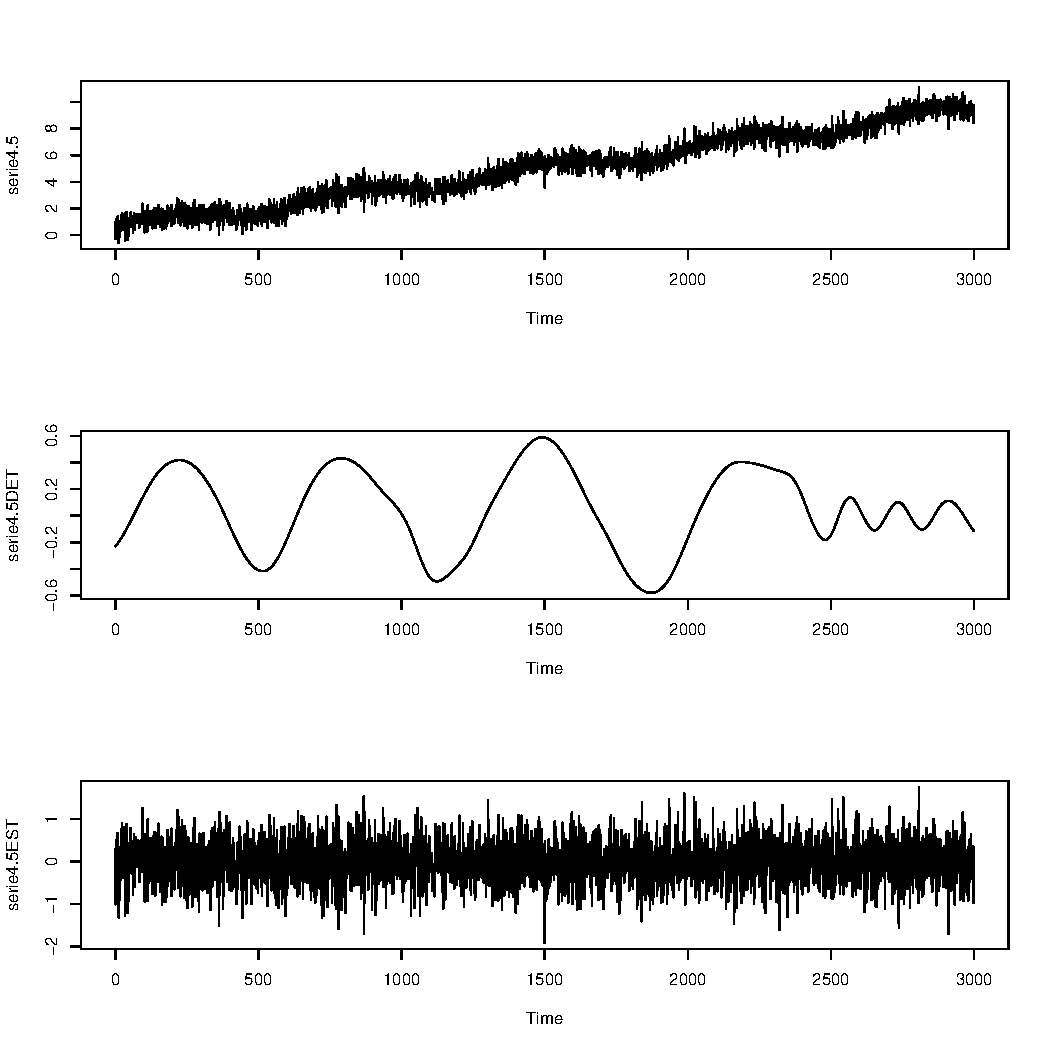
\includegraphics[scale=0.43]{serie4_5.pdf} \quad
  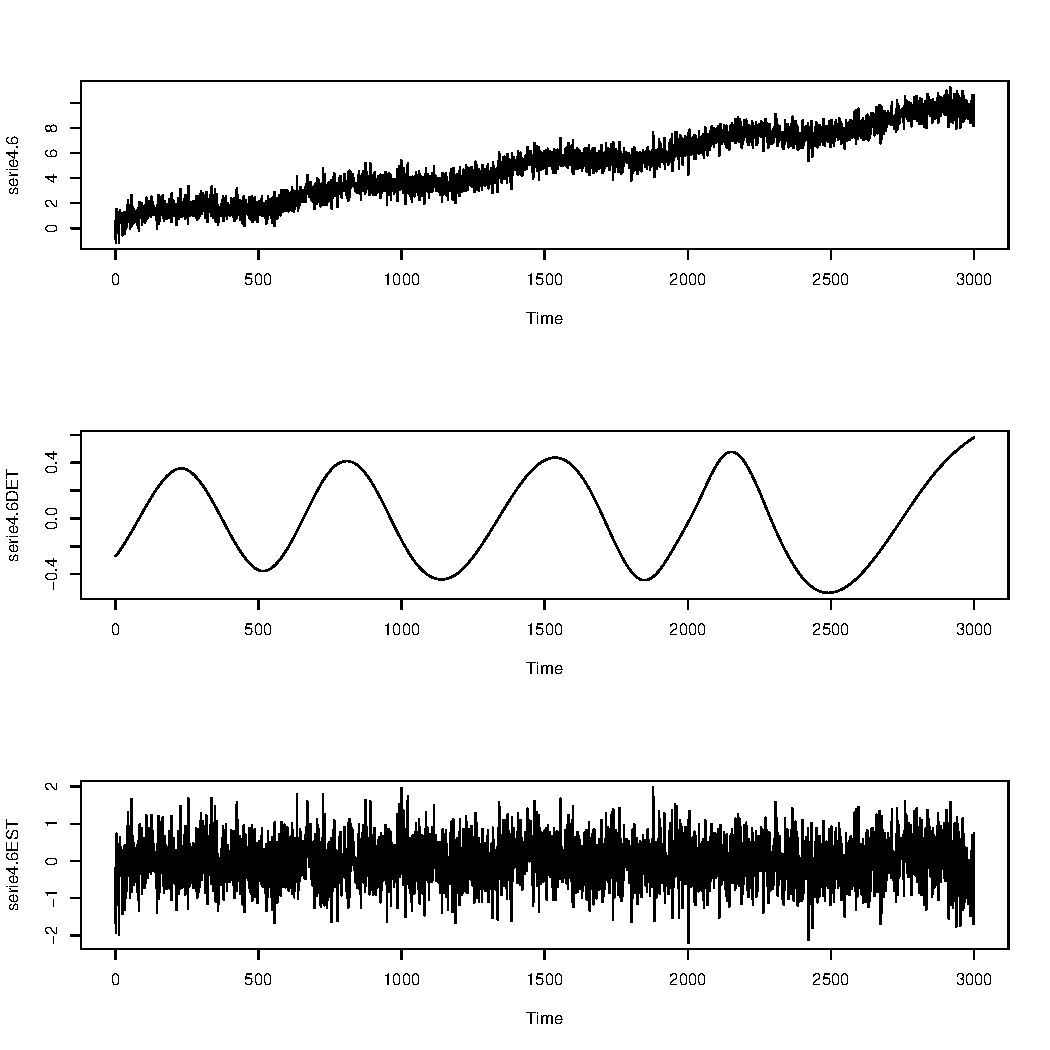
\includegraphics[scale=0.43]{serie4_6.pdf}
 \caption{Série 4.5 e Série 4.6}

\end{center}
\end{figure}

\graphicspath{{imagens/}}
\begin{figure}[H]
\begin{center}
  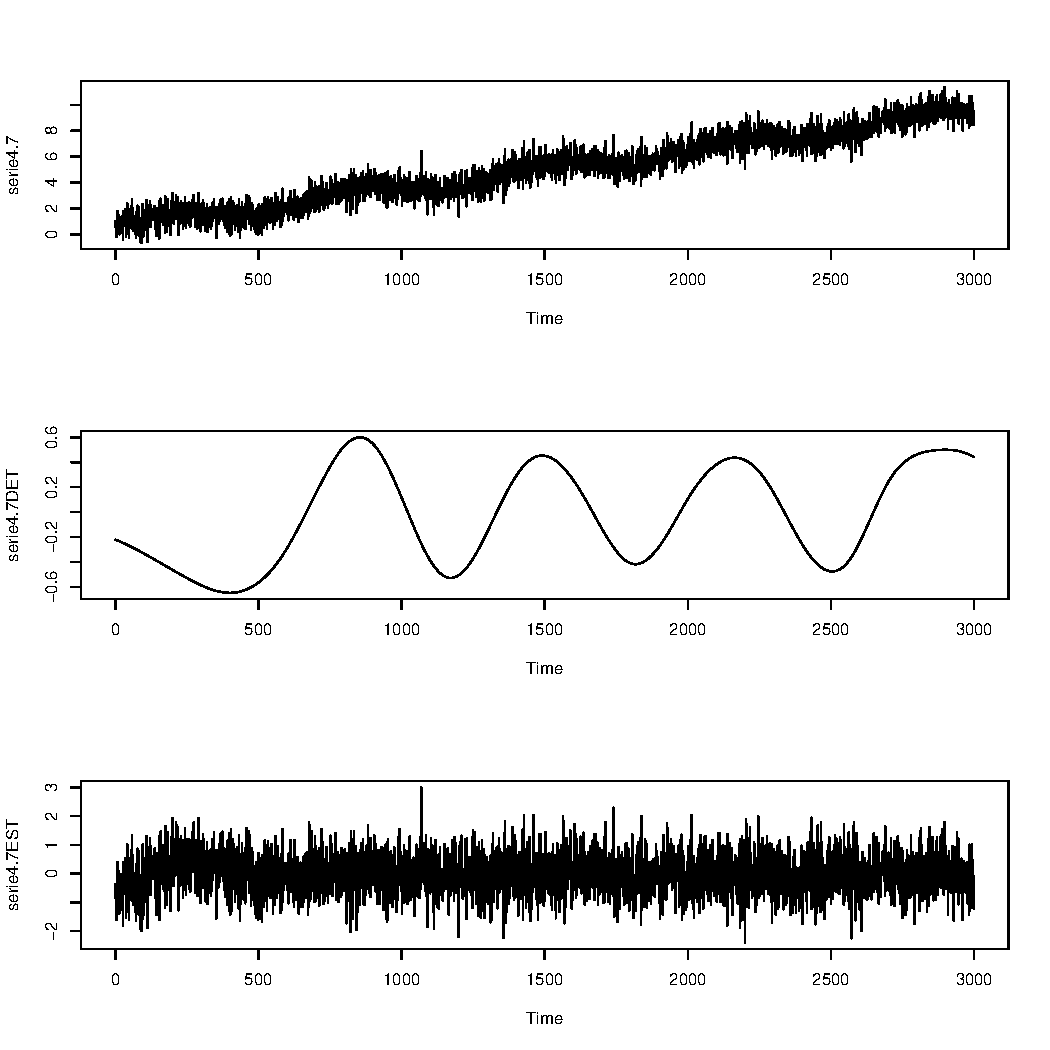
\includegraphics[scale=0.43]{serie4_7.pdf} \quad
  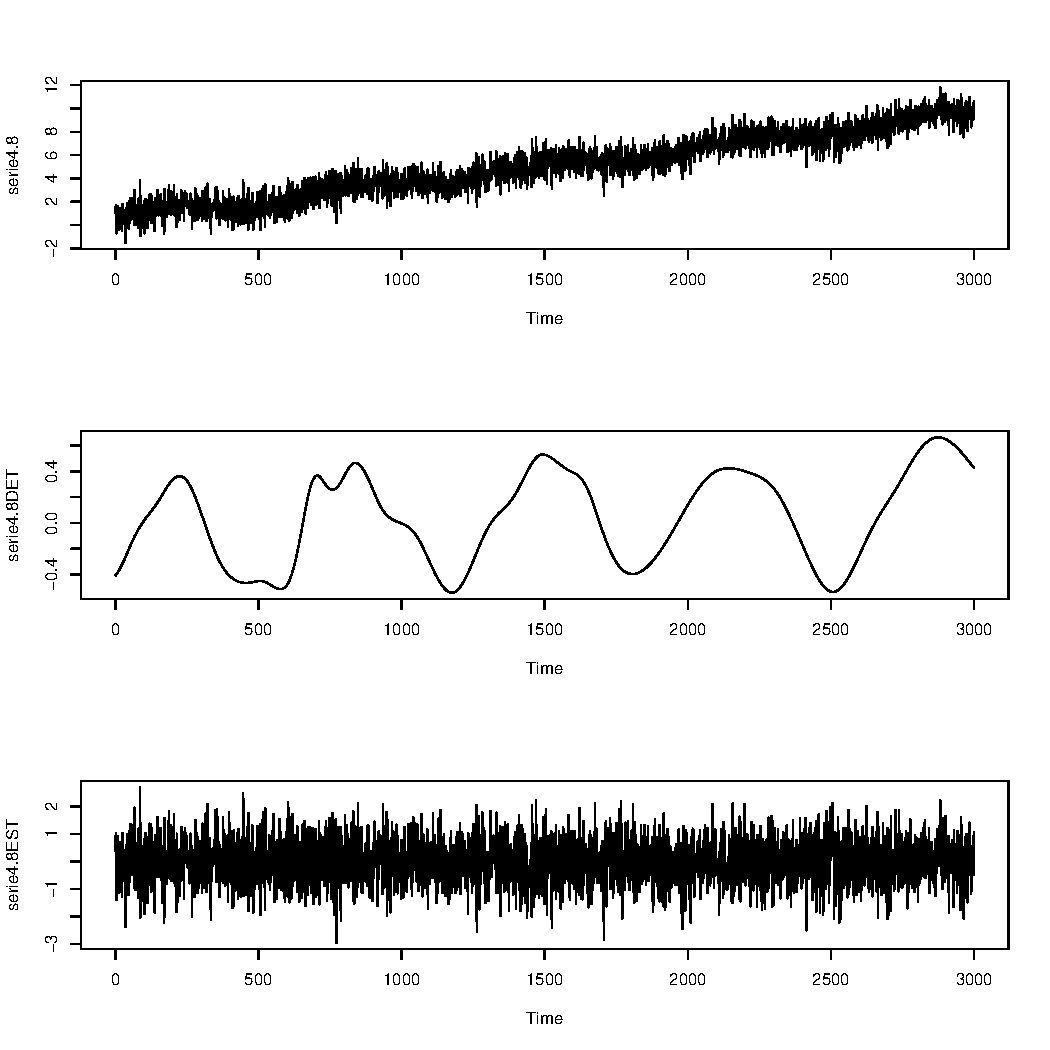
\includegraphics[scale=0.43]{serie4_8.pdf}
  \caption{Série 4.7 e Série 4.8}

\end{center}
\end{figure}

\graphicspath{{imagens/}}
\begin{figure}[H]
\begin{center}
  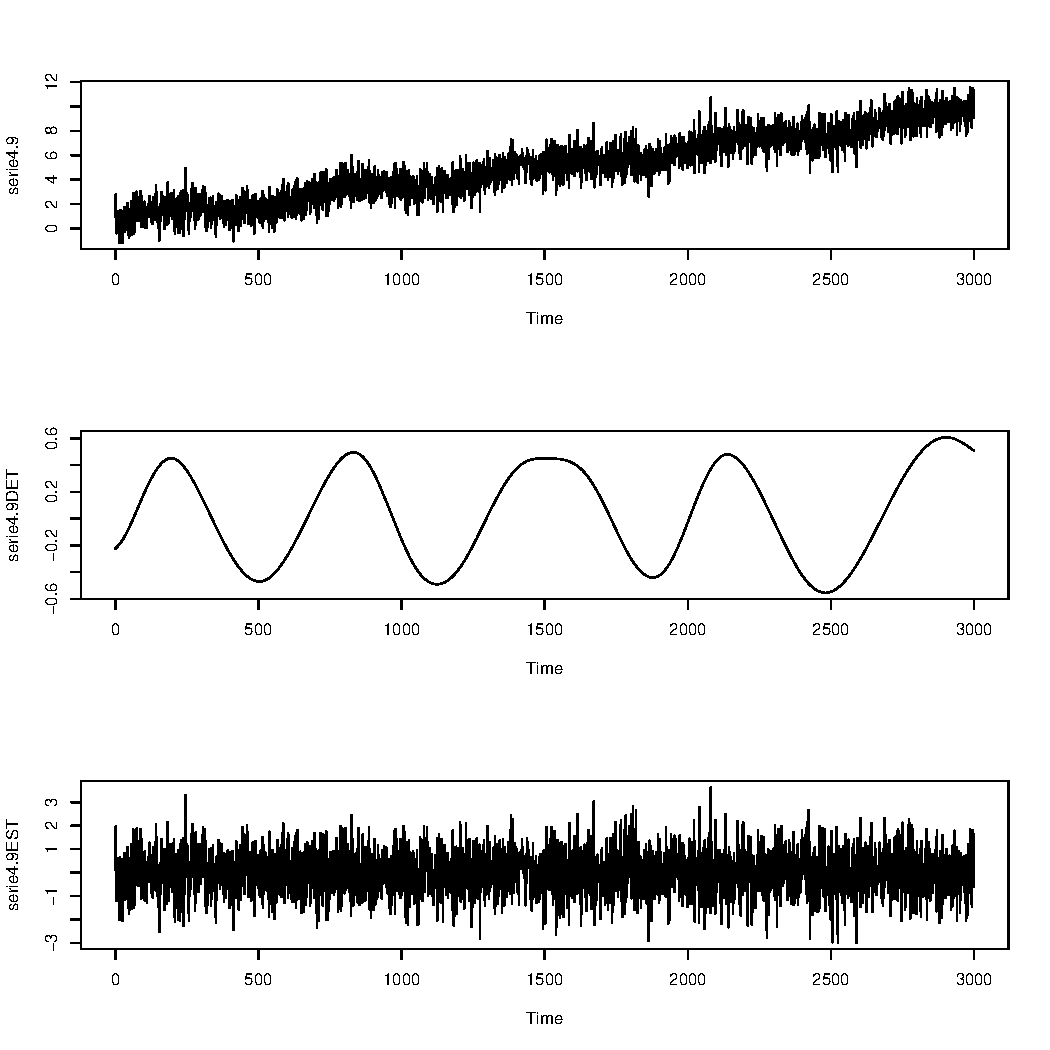
\includegraphics[scale=0.43]{serie4_9.pdf} \quad
  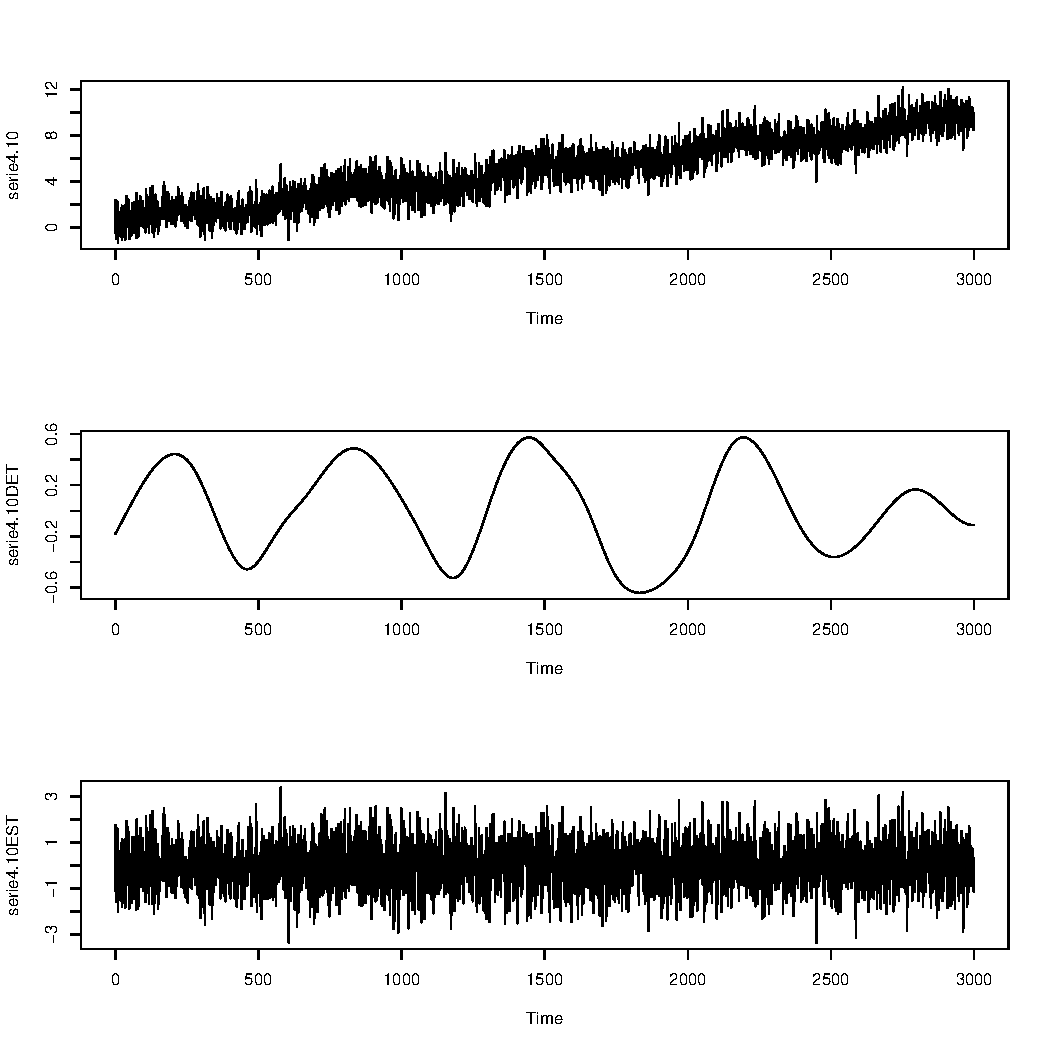
\includegraphics[scale=0.43]{serie4_10.pdf}
  \caption{Série 4.9 e Série 4.10}
\end{center}
\end{figure}
\section{Considerações Finais}
Foram apresentadas as séries temporais utilizadas neste trabalho experimental e suas respactivas decomposições.
% \include{apendice2}
% ...
% \include{apendiceM}

%% Fim do documento
\end{document}
%------------------------------------------------------------------------------------------%
